\chapter{Supplements: PixArt-$\Sigma$ Experiments}

\section{Experimental Default Setup}
Tab. \ref{tab:hyperparameterTraining} presents the default fine-tuning settings used for PixArt-$\Sigma$. To speed up the training process, the embeddings of the images and the text prompts are pre-computed and stored on disk. Since the image size in the LAION5B dataset vary, the images were resized such that the shortest edge has the size of 512. Then, the image is cropped in the center to extract an image of exactly the size of $512 \times 512$. This crop is then encoded by the \gls{VAE} and the embeddings are stored. 

In general, BF16 precision was used to reduce memory requirements and further speed up the training process. FP32 precision was used only for the attention computation, as the authors otherwise observed training instabilities..

\begin{table}[H]
	\centering
	\caption[PixArt-$\Sigma$ Fine-Tuning Hyperparameters]{Default hyperparameter settings for PixArt-$\Sigma$ fine-tuning after compression.}
	\label{tab:hyperparameterTraining}
	\begin{tabular}{l c}
		\toprule
		\textbf{Hyperparameter} & \textbf{Value} \\
		\midrule
		\multicolumn{2}{l}{\textit{\textbf{Optimization}}} \\
		\midrule
		Optimizer Type & CAME \\
		Learning Rate & $2 \times 10^{-5}$ (Block Removal)/ $2 \times 10^{-6}$ (SVD Compression)\\
		Weight Decay & $0.03$ \\
		Betas & $(0.9, 0.999, 0.9999)$ \\
		Epsilon & $(10^{-30}, 10^{-16})$ \\
		\midrule
		\multicolumn{2}{l}{\textit{\textbf{Training Schedule}}} \\
		\midrule
		Warmup Steps & 1000 \\
		Batch Size & 16 \\
		Gradient Clipping & $0.001$ \\
		\midrule
		\multicolumn{2}{l}{\textit{\textbf{Model \& Data}}} \\
		\midrule
		Precision & bf16 \\
		Attention Precision & FP32 \\
		Resolution & $512 \times 512$ \\
		Class Dropout Prob. & $0.1$ \\
		Max Prompt Length & 300 \\
		\bottomrule
	\end{tabular}
\end{table}

\section{Block Importance Analysis}
The heatmap of the \gls{CKA} scores across all PixArt-$\Sigma$ blocks and timesteps is displayed in Fig. \ref{fig:PixArtBlockImportanceHeatmap}. It demonstrates that the \gls{CKA} score can vary significantly for a single block over the course of the image generation trajectory (e.g. block 22), indicating that blocks have varying importance at different timesteps. Furthermore, this section provides the complete set of images for the qualitative analysis of block compression by 60\% (Fig. \ref{fig:AppxPixArtCMMDCompression})

\subsubsection{CKA-Analysis of Transformer Blocks}

\begin{figure}[H]
	\centering
	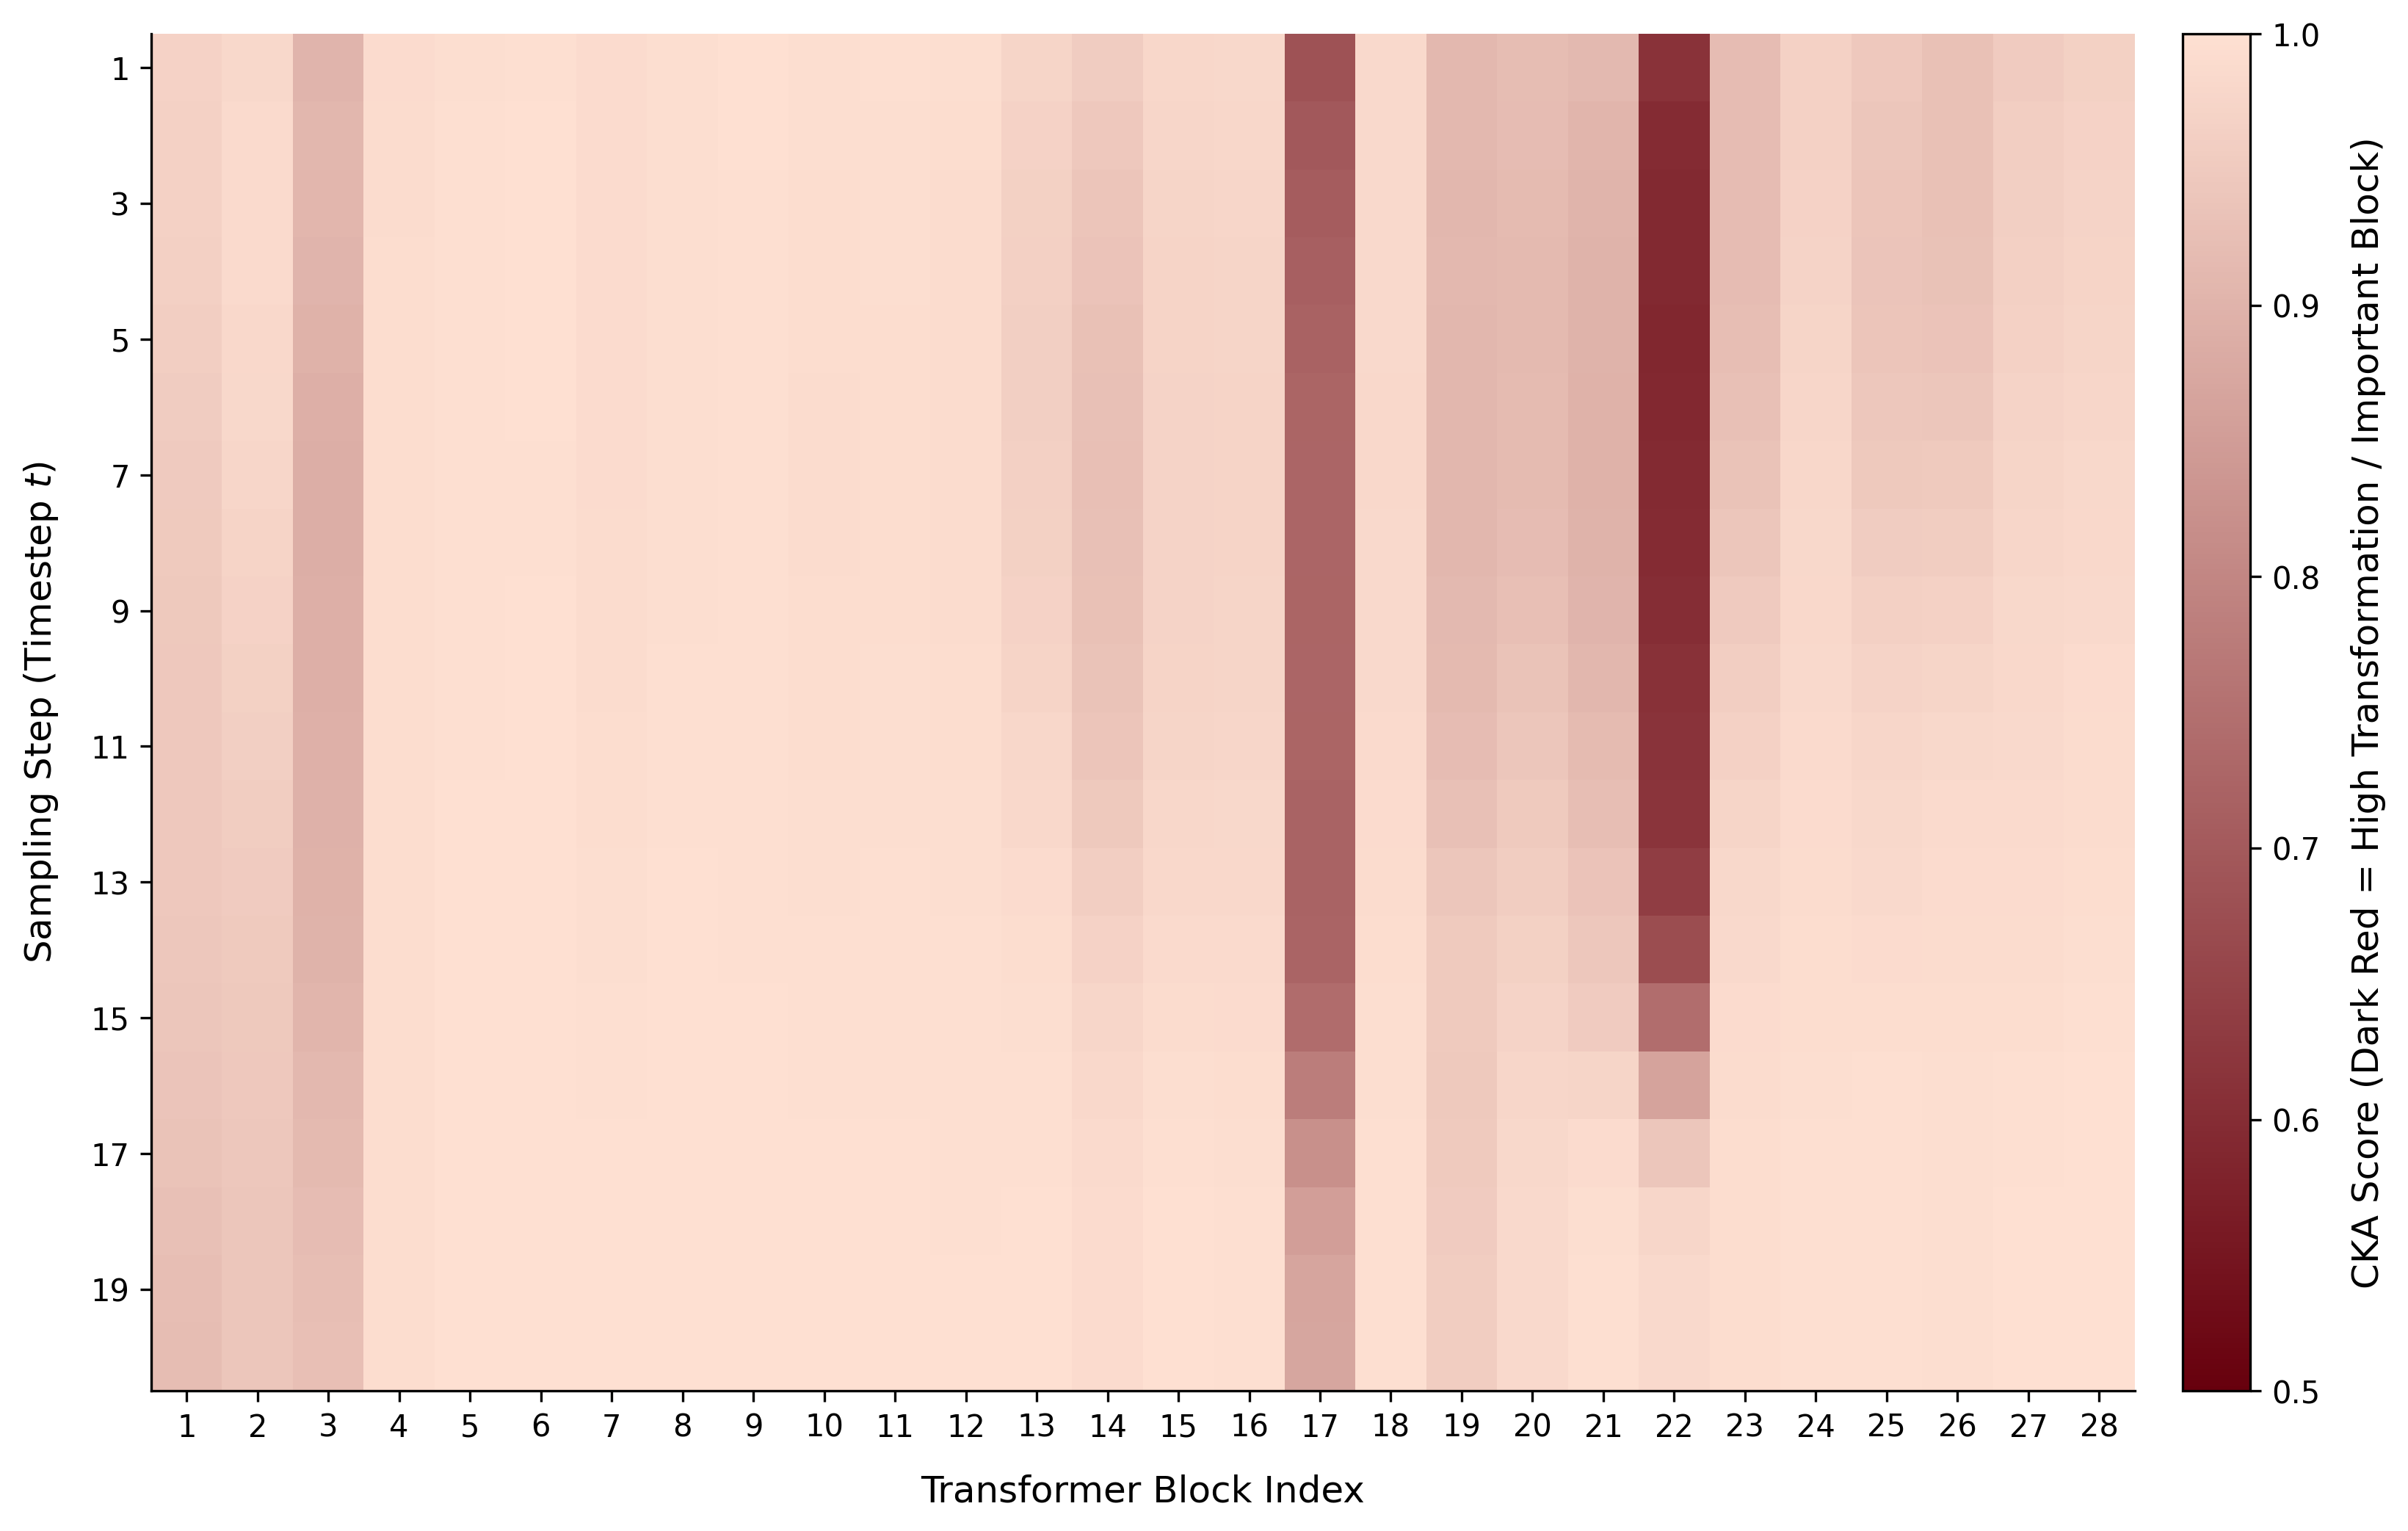
\includegraphics[width=0.65\textwidth]{images/Experimente/Pixart_Block_Analysis/cka_heatmap_100_thesis.png}  % adjust filename and width
	\caption[CKA-Score Heatmap]{The heatmap displays the \gls{CKA} score for all PixArt-$\Sigma$ blocks across all timesteps.}
	
	\label{fig:PixArtBlockImportanceHeatmap}
\end{figure}

\subsubsection{Qualitative Block Selection Analysis}
\begin{figure}[H]
	\centering
	
\includegraphics[width=0.7\textwidth]{images/Experimente/PixArt_Block_Analysis/BlockAnalysisCompression06.pdf}  % adjust filename and width
	\caption[Qualitative Block Importance Analysis of PixArt-$\Sigma$: Block Compression]{Illustration of the impact of selectively compressing individual Transformer blocks (1–28) by 60\% on the final generation result.}
	
	\label{fig:AppxPixArtCMMDCompression}
\end{figure}




\section{One-Shot vs. Progressive Model Compression}
\label{sec:OneShotVsProgressivePrunAppendix}
Tab. \ref{tab:SettingOneShotvsProgressive} details the technical settings for the experiments comparing one-shot and progressive model pruning (Sec. \ref{sec:OneShot_vs_Progrosseve_Pruning}).
Moreover, this section presents qualitative example images generated by models compressed to various ratios (Figs. \ref{fig:FinetuningProtocol_Appx90} - \ref{fig:FinetuningProtocol_60}). These images were obtained using the one-shot and progressive pruning approaches, as detailed in Section \ref{sec:OneShot_vs_Progrosseve_Pruning}. Note that for the model pruned to 90\%, the one-shot and progressive pruning schedules are identical.


\begin{table}[H]
	\centering
	\caption[Block Removal Details: One-Shot vs. Progressive Pruning]{Overview of the compression details utilized for the one-shot and progressive pruning experiments on the PixArt-$\Sigma$ model.}
	\label{tab:SettingOneShotvsProgressive}
	\begin{tabular}{@{} l c c c @{}}
		\toprule
		\textbf{Model Variant} & \textbf{Number of}  & \textbf{Training Steps} \\
		\textbf{(Remaining \%)} & \textbf{Removed Blocks}  & \textbf{(in Thousands)} \\
		\midrule
		Model 90\% & 3 & 88.5 \\
		Model 80\% & 6   & 265.5 \\
		Model 70\% & 8   & 531.0 \\
		Model 60\% & 11  & 708.0 \\
		Model 50\% & 14  & 973.5 \\
		\bottomrule
	\end{tabular}
	
\end{table}




\begin{figure}[H]
	\centering
	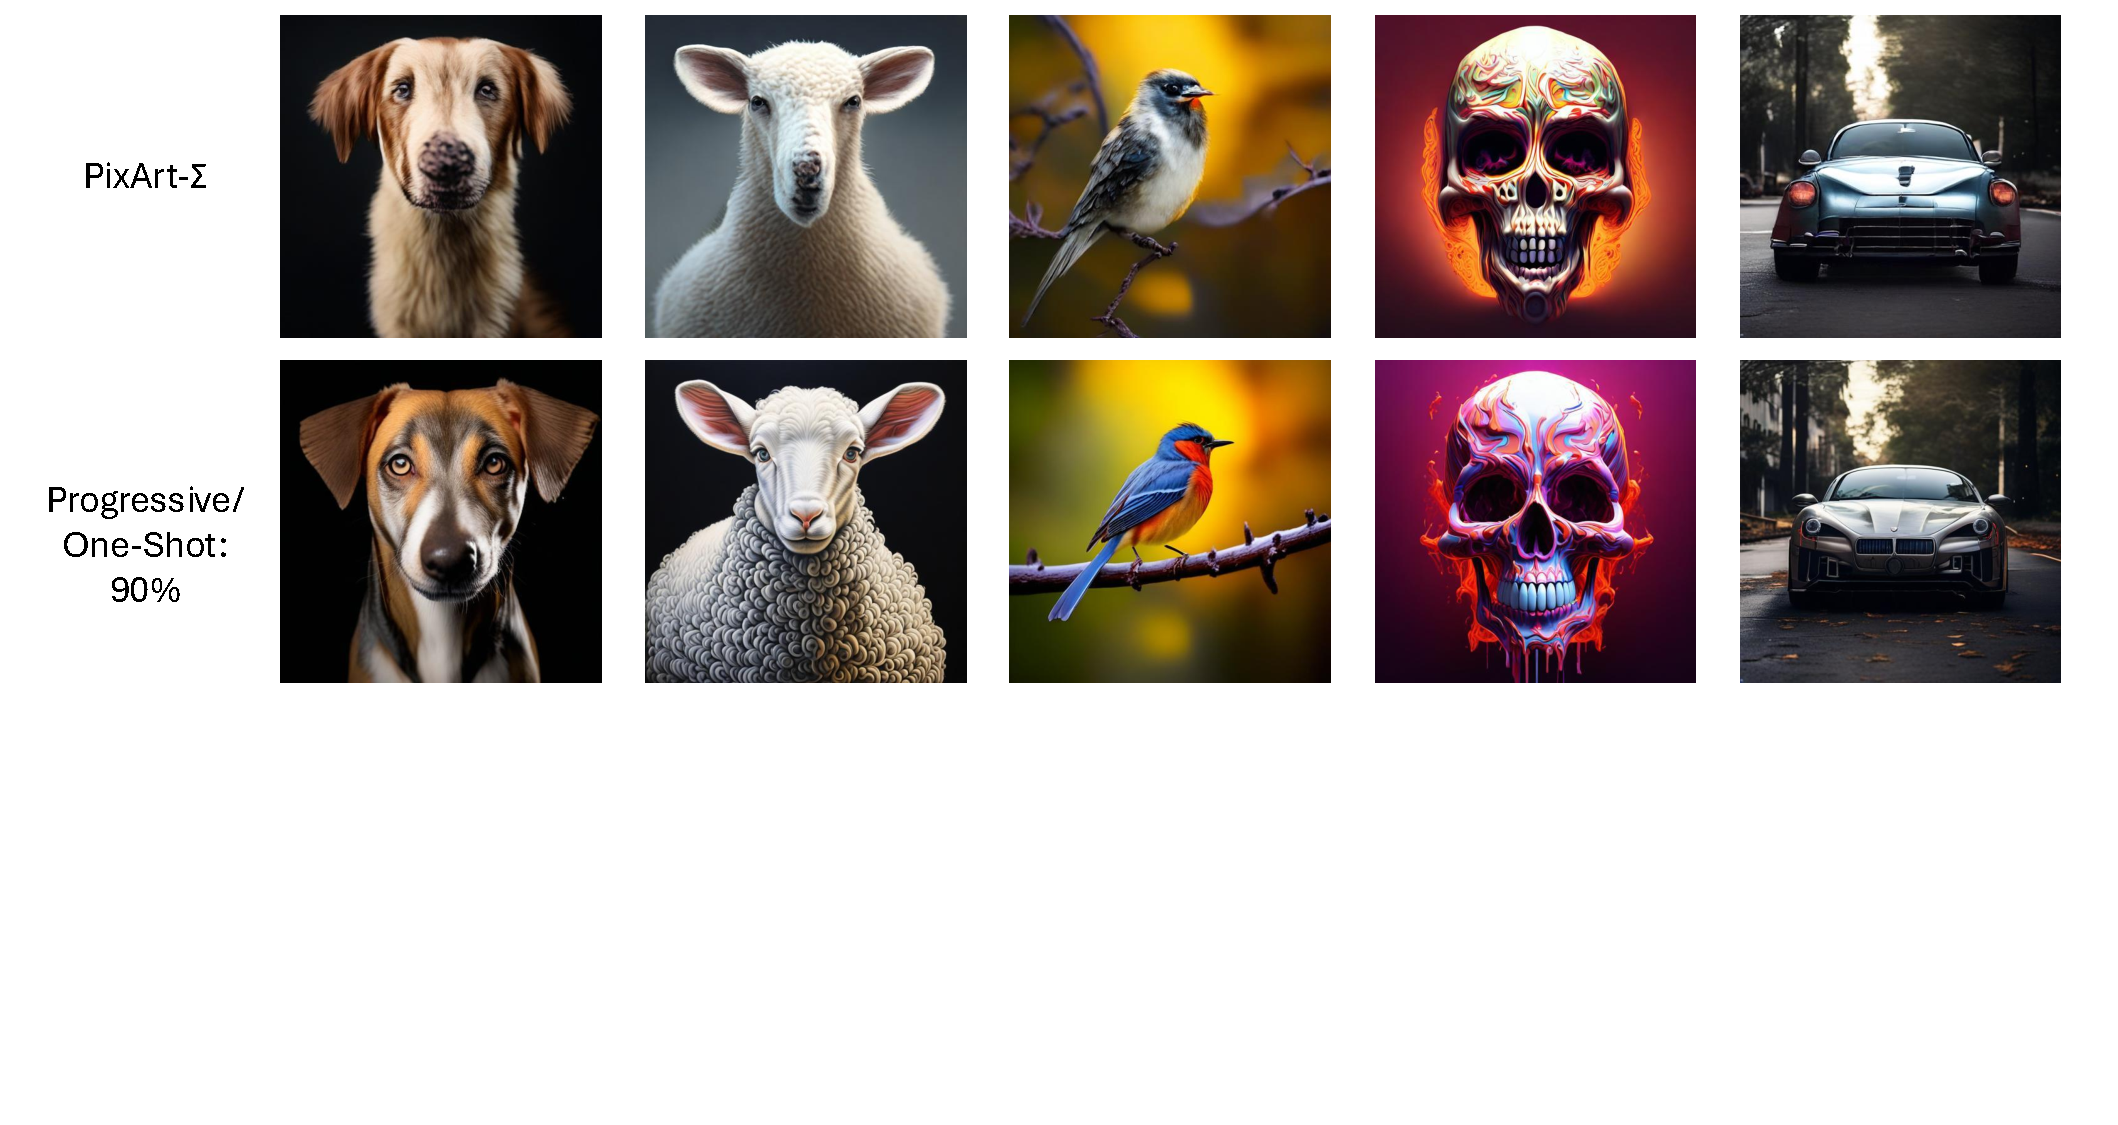
\includegraphics[width=0.7\textwidth]{images/Experimente/Iterative_vs_Direct/Examples_model_90.pdf}
	\caption[Qualitative Examples: One-Shot vs. Progressive Model Pruning (90\% Model)]{Qualitative comparison of example images generated by models reduced to 90\% using either a one-shot or a progressive compression strategy.}
	\label{fig:FinetuningProtocol_Appx90}
\end{figure}


\begin{figure}[H]
	\centering
	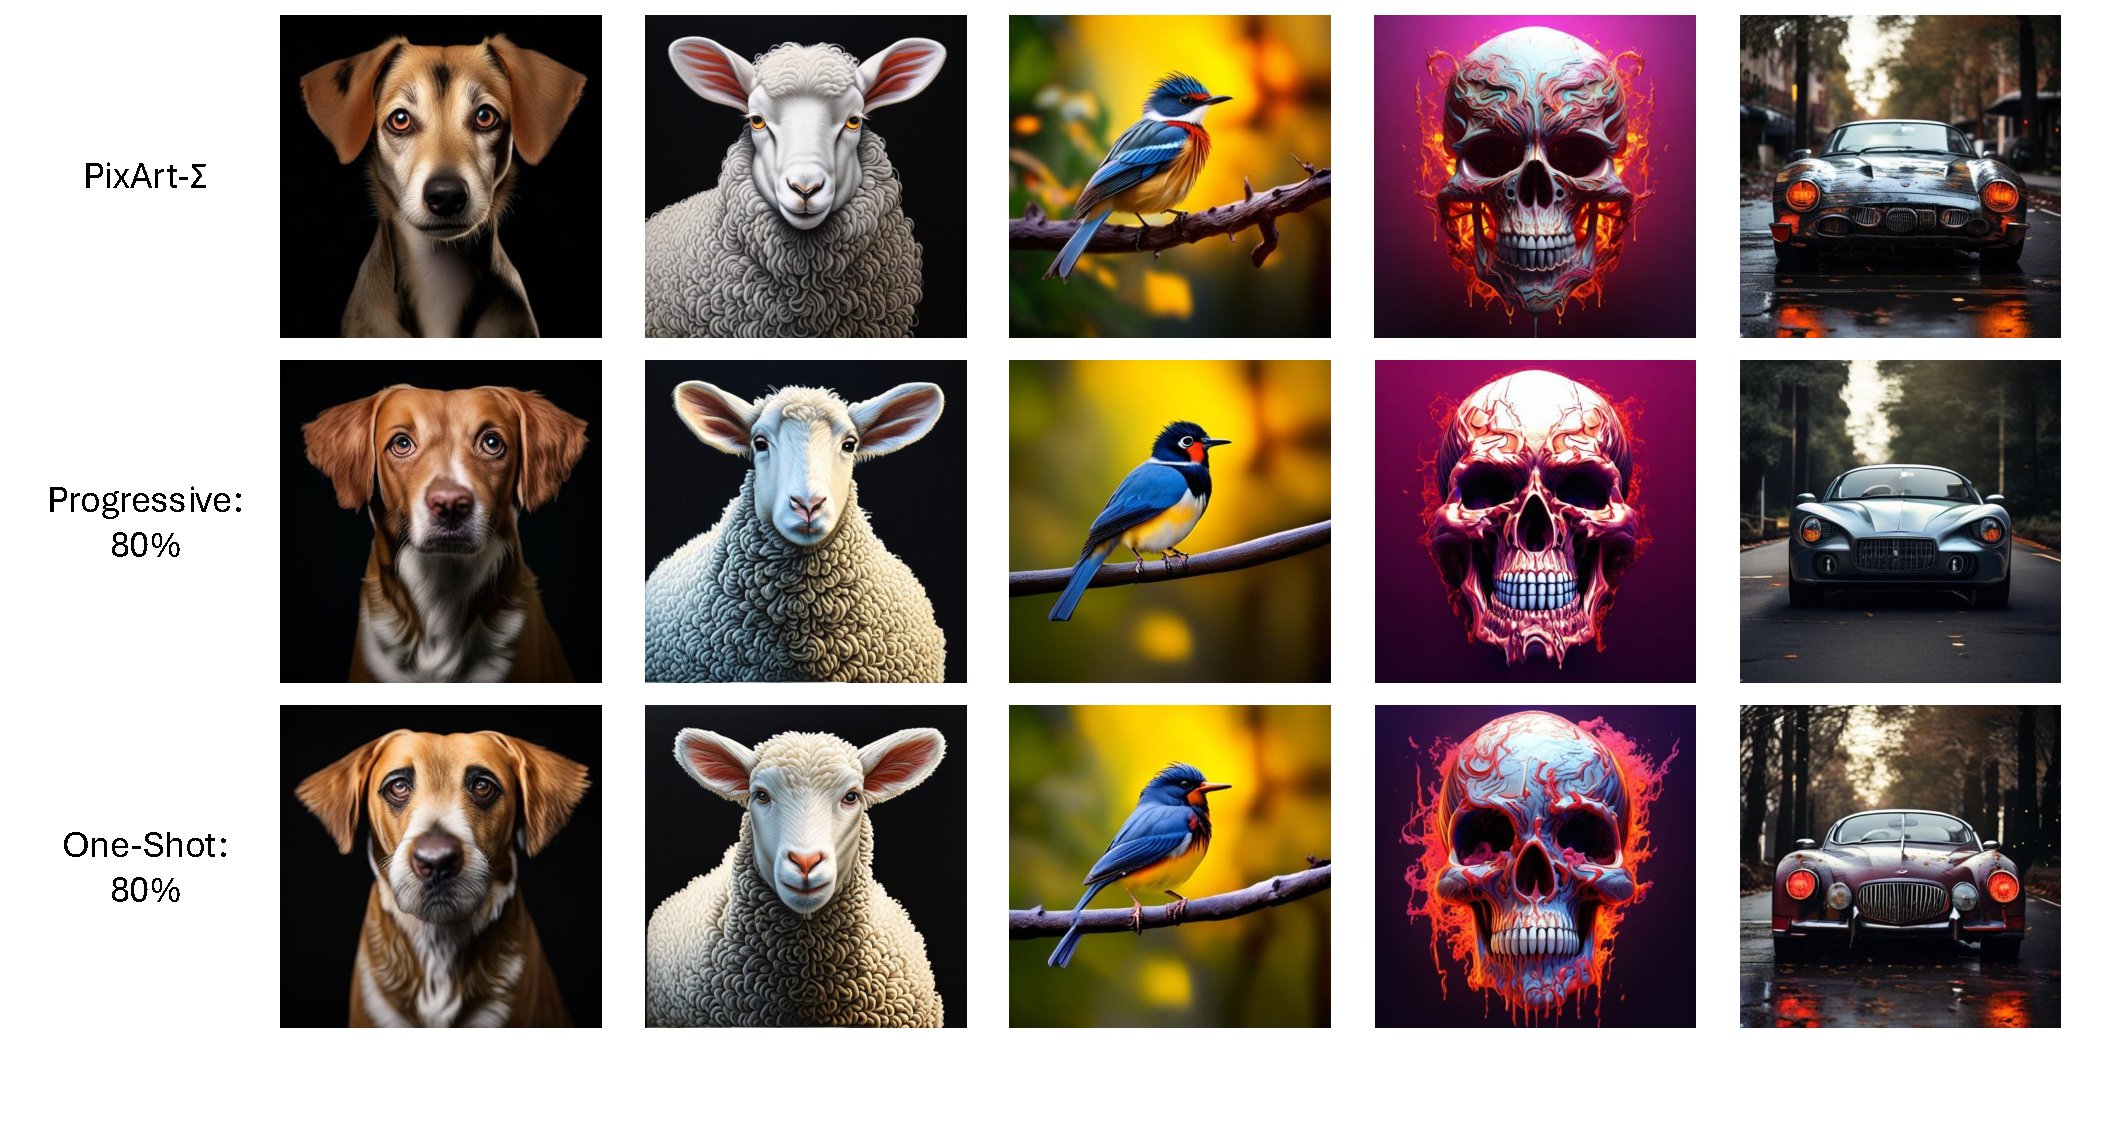
\includegraphics[width=0.7\textwidth]{images/Experimente/Iterative_vs_Direct/Examples_model_80.pdf}
	\caption[Qualitative Examples: One-Shot vs. Progressive Model Pruning (80\% Model)]{Qualitative comparison of example images generated by models reduced to 80\% using either a one-shot or a progressive compression strategy.}
	\label{fig:FinetuningProtocol_Appx80}
\end{figure}

\begin{figure}[H]
	\centering
	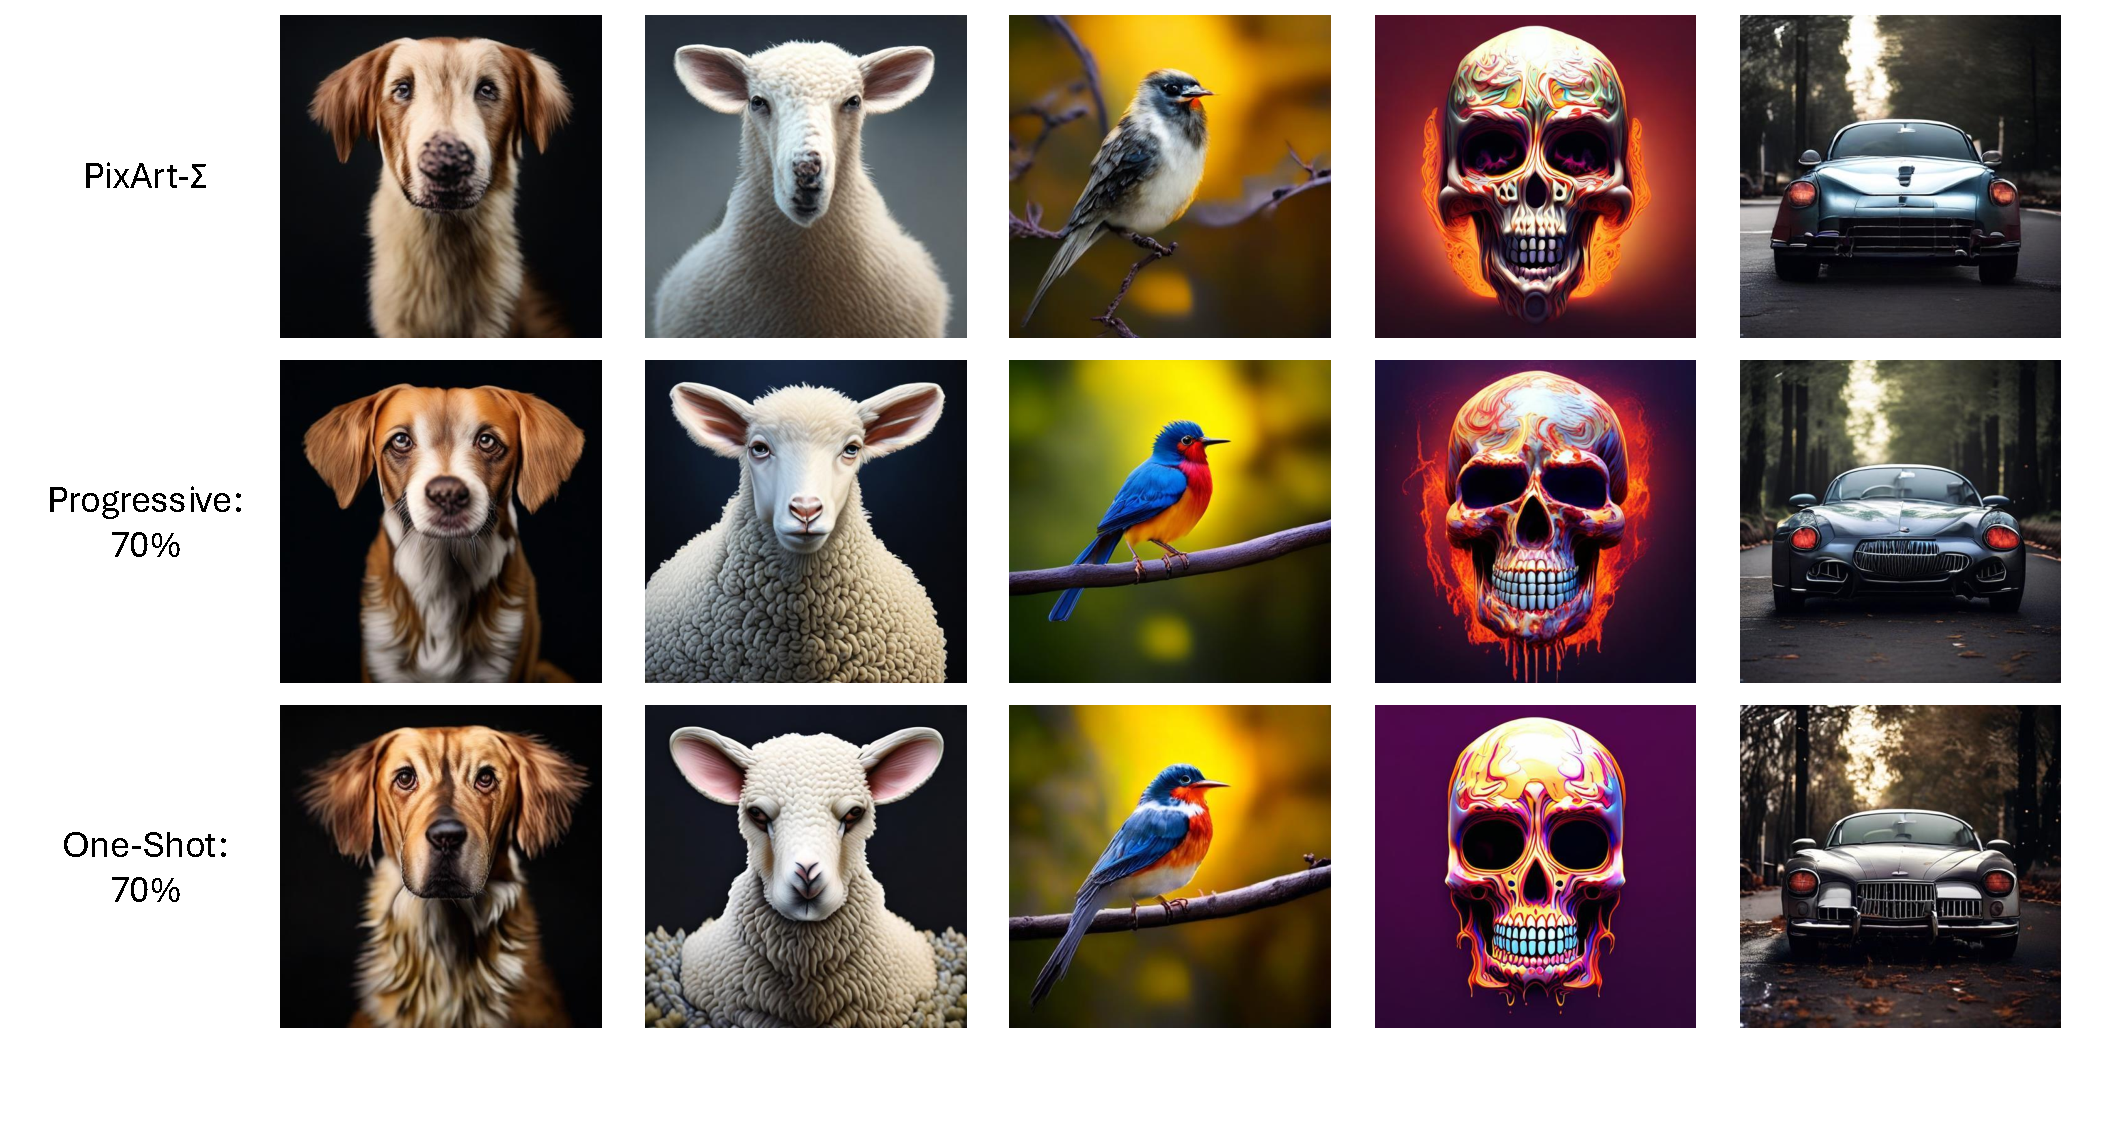
\includegraphics[width=0.7\textwidth]{images/Experimente/Iterative_vs_Direct/Examples_model_70.pdf}
	\caption[Qualitative Examples: One-Shot vs. Progressive Model Pruning (70\% Model)]{Qualitative comparison of example images generated by models reduced to 70\% using either a one-shot or a progressive compression strategy.}
	\label{fig:FinetuningProtocol_70}
\end{figure}

\begin{figure}[H]
	\centering
	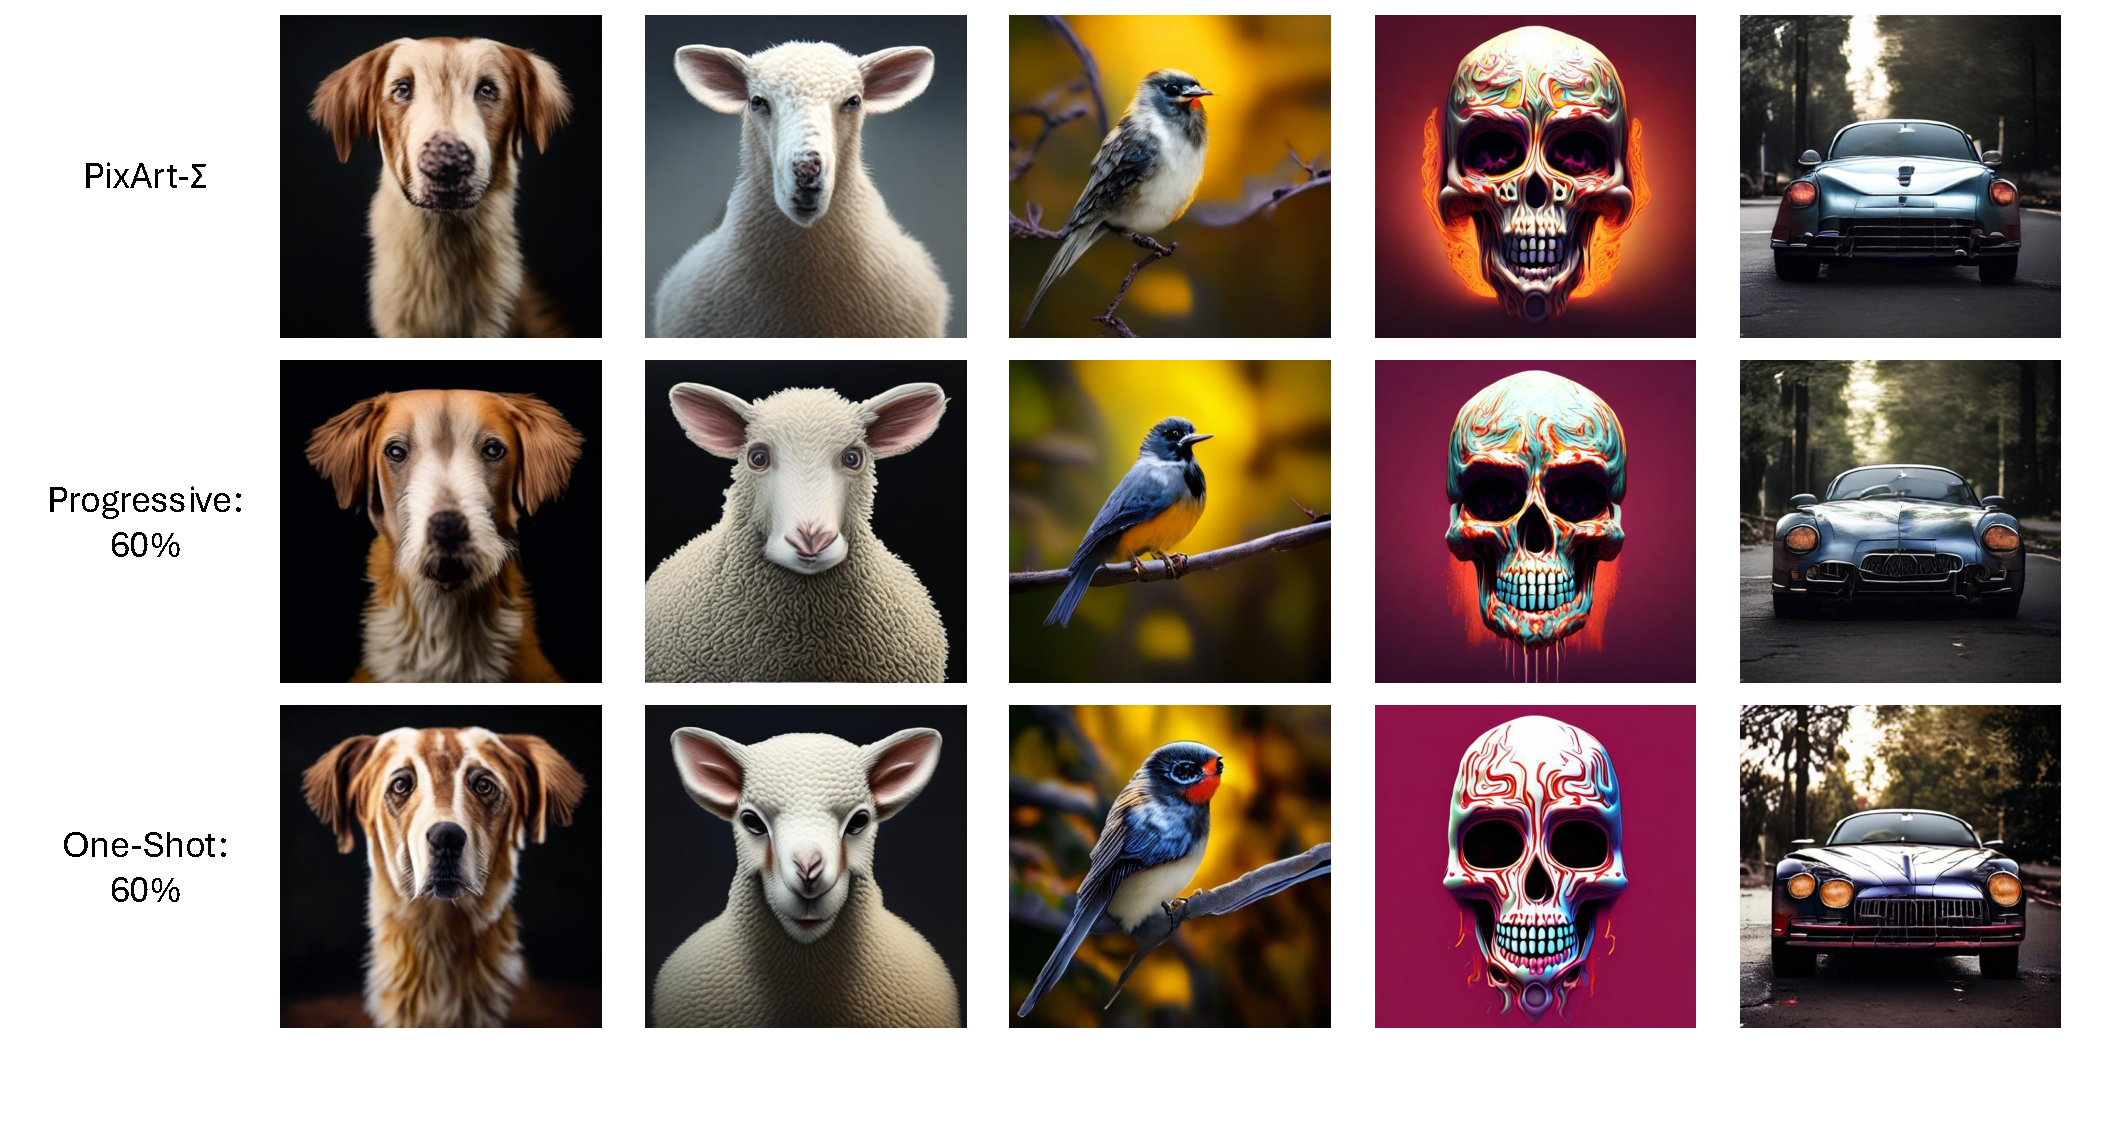
\includegraphics[width=0.7\textwidth]{images/Experimente/Iterative_vs_Direct/Examples_model_60.pdf}
	\caption[Qualitative Examples: One-Shot vs. Progressive Model Pruning (60\% Model)]{Qualitative comparison of example images generated by models reduced to 60\% using either a one-shot or a progressive compression strategy.}
	\label{fig:FinetuningProtocol_60}
\end{figure}

\section{Knowledge Distillation Loss}
\label{sec:KnowledgeDistillationAppendix}
This section provides an analysis of the average feature magnitudes across individual PixArt-$\Sigma$ Transformer blocks, measured via the \gls{RMS} norm (Fig. \ref{fig:MagnitudeIntermediateFeatures}). Additionally, this section presents qualitative examples comparing various knowledge distillation loss configurations (Sec. \ref{sec:ExpKDLoss}) across several model compression ratios (Figs. \ref{fig:QualitativeLossInvestigation_90} - \ref{fig:QualitativeLossInvestigation_50}).

\begin{figure}[H]
	\centering
	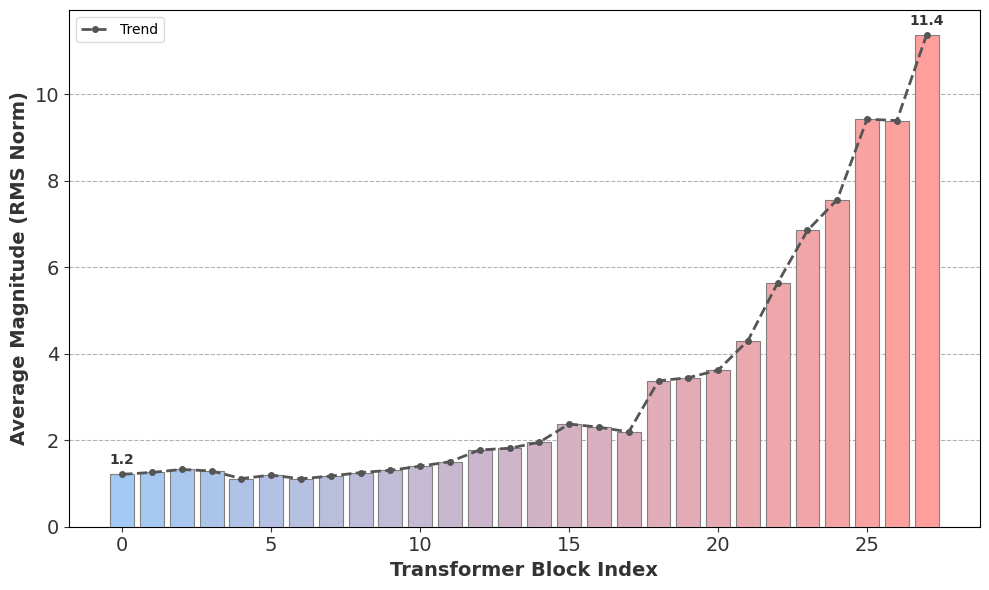
\includegraphics[width=0.6\textwidth]{images/Experimente/loss_investigation/magnitude_block_features.png}  
	\caption[Magnitude of Intermediate Features in PixArt-$\Sigma$]{The \gls{RMS} norm of output features across individual PixArt-$\Sigma$ Transformer blocks exhibits significant variance, with later layers generally displaying larger magnitudes than preceding ones. Results are averaged over 100 prompts from the LAION dataset.}
	\label{fig:MagnitudeIntermediateFeatures}
\end{figure}


\begin{figure}[H]
	\centering
	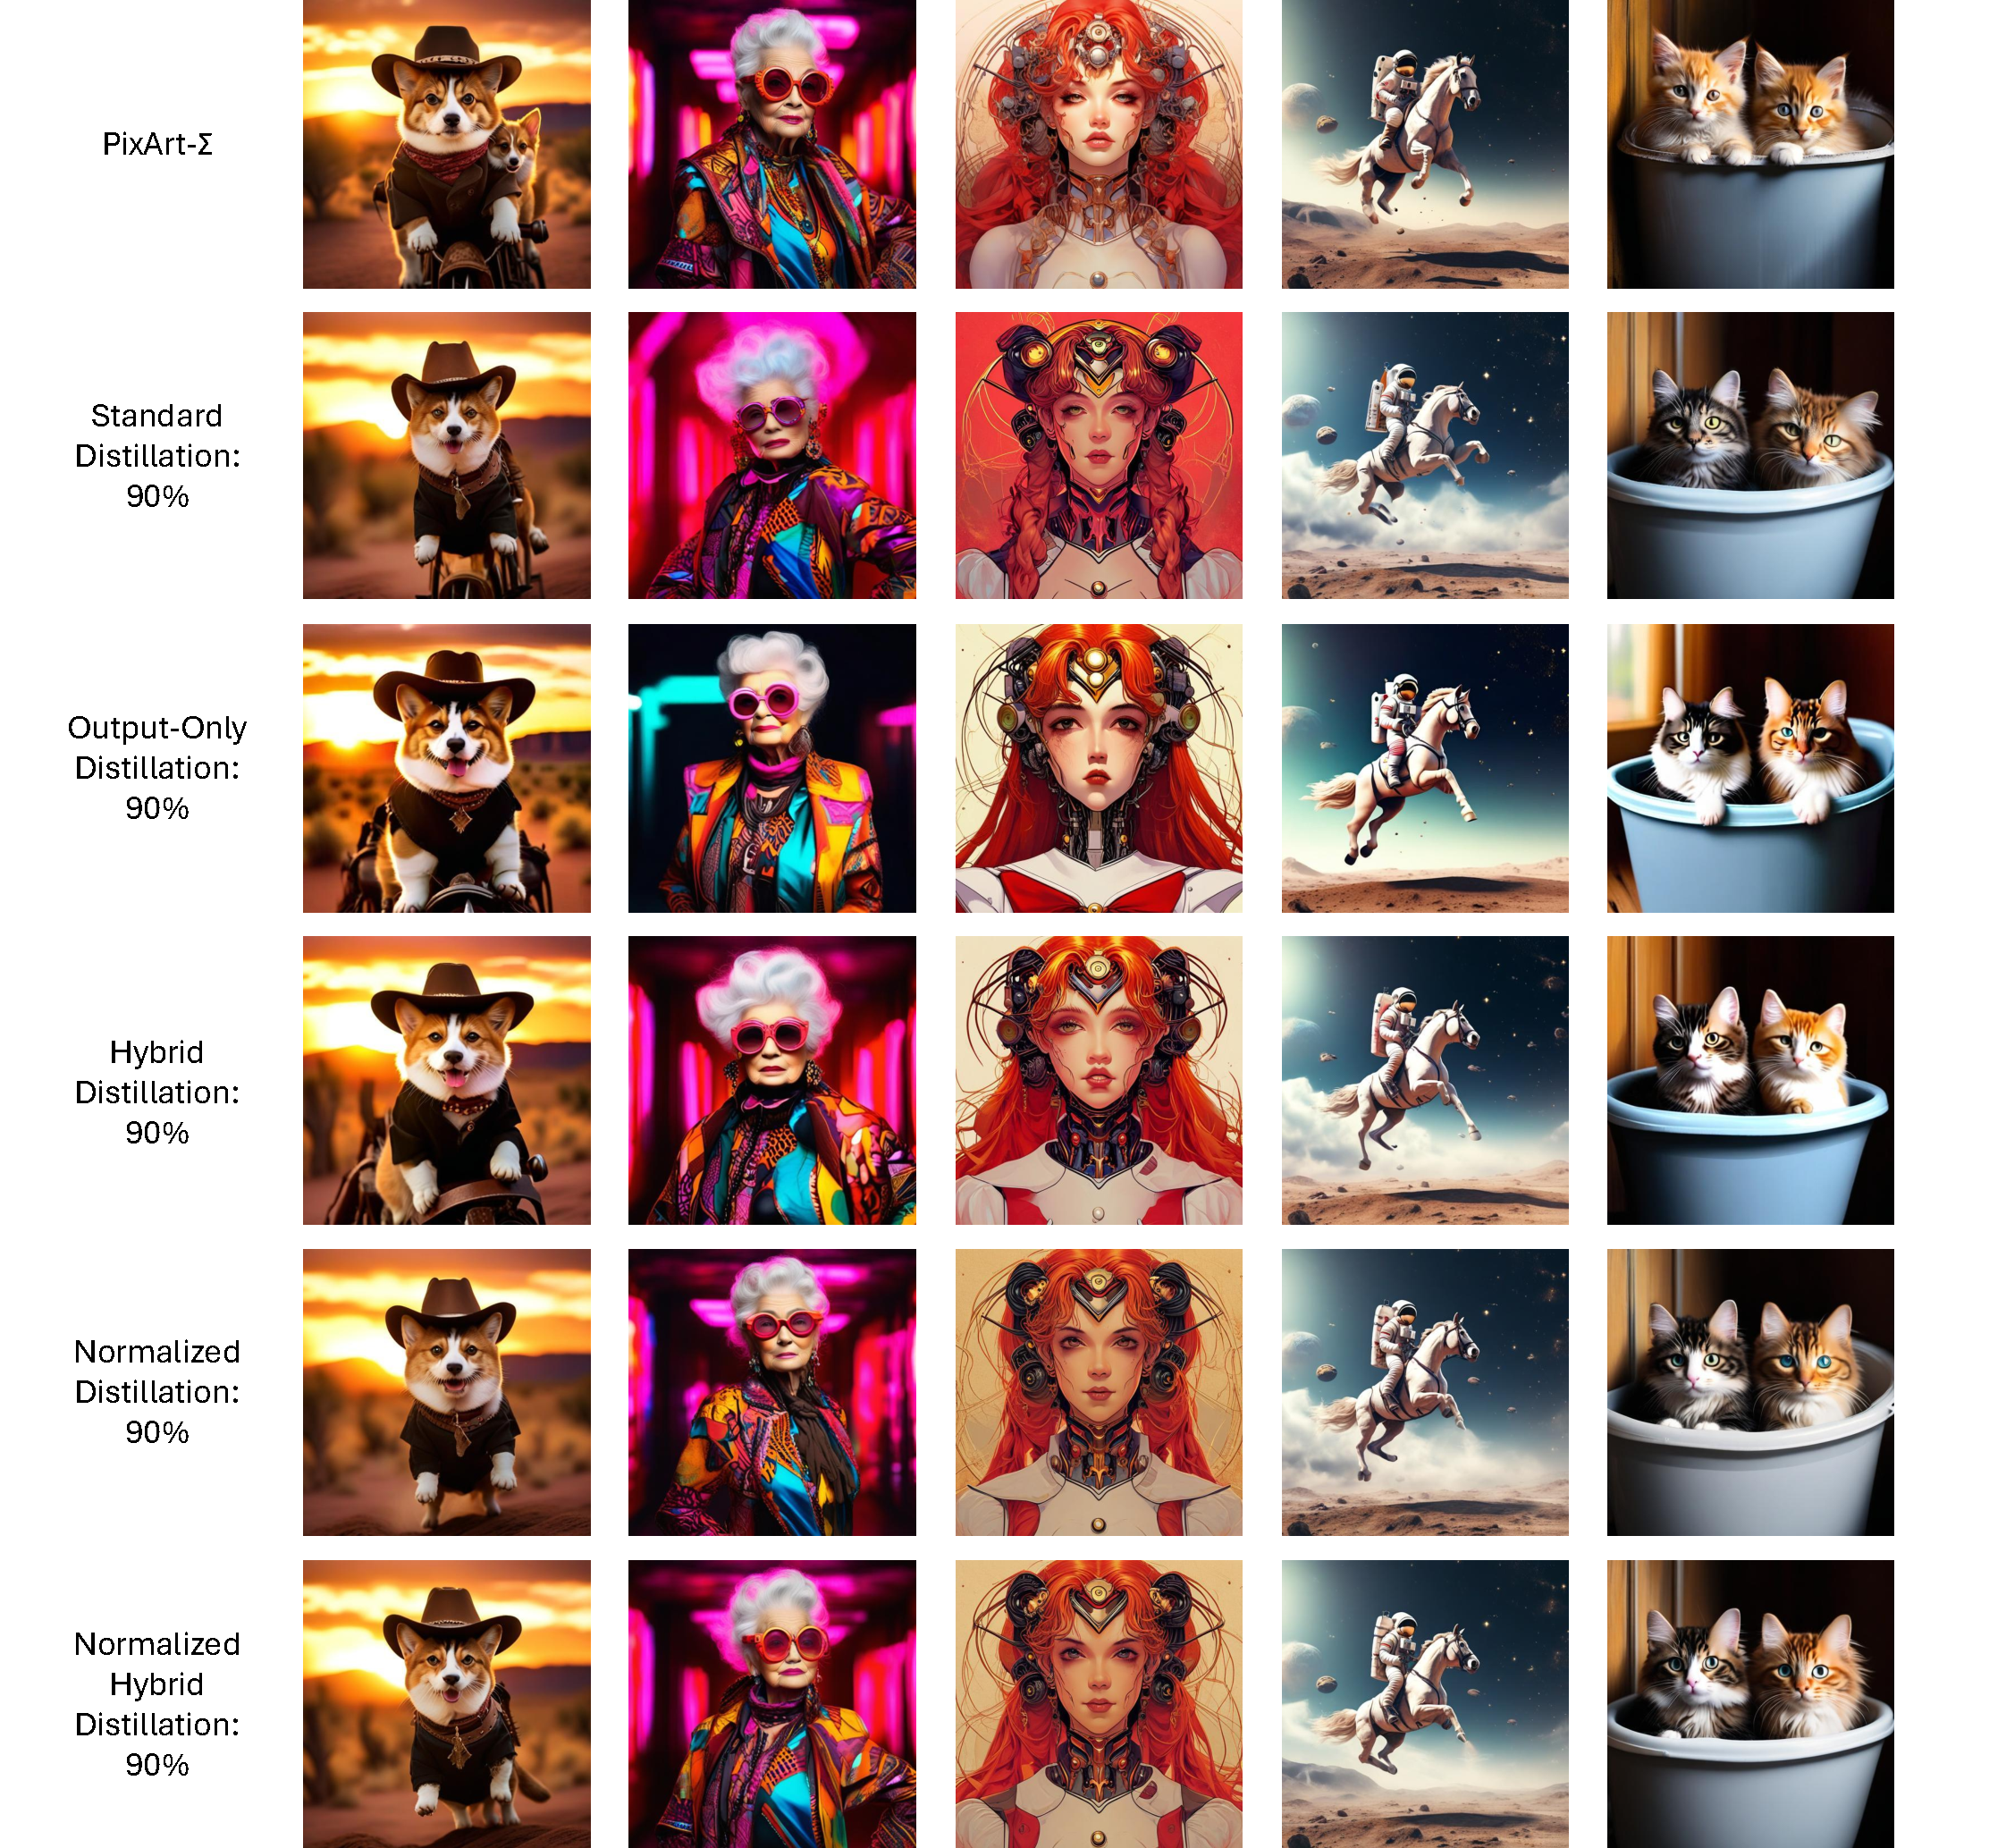
\includegraphics[width=0.65\textwidth]{images/Appendix/KnowledgeDistillation/model_90.pdf}
	\caption[Qualitative Examples: Different Knowledge Distillation Loss Configurations (90\% Model)]{Qualitative comparison of example images generated by models compressed to 90\% using various knowledge distillation loss configurations}
	\label{fig:QualitativeLossInvestigation_90}
\end{figure}

\begin{figure}[H]
	\centering
	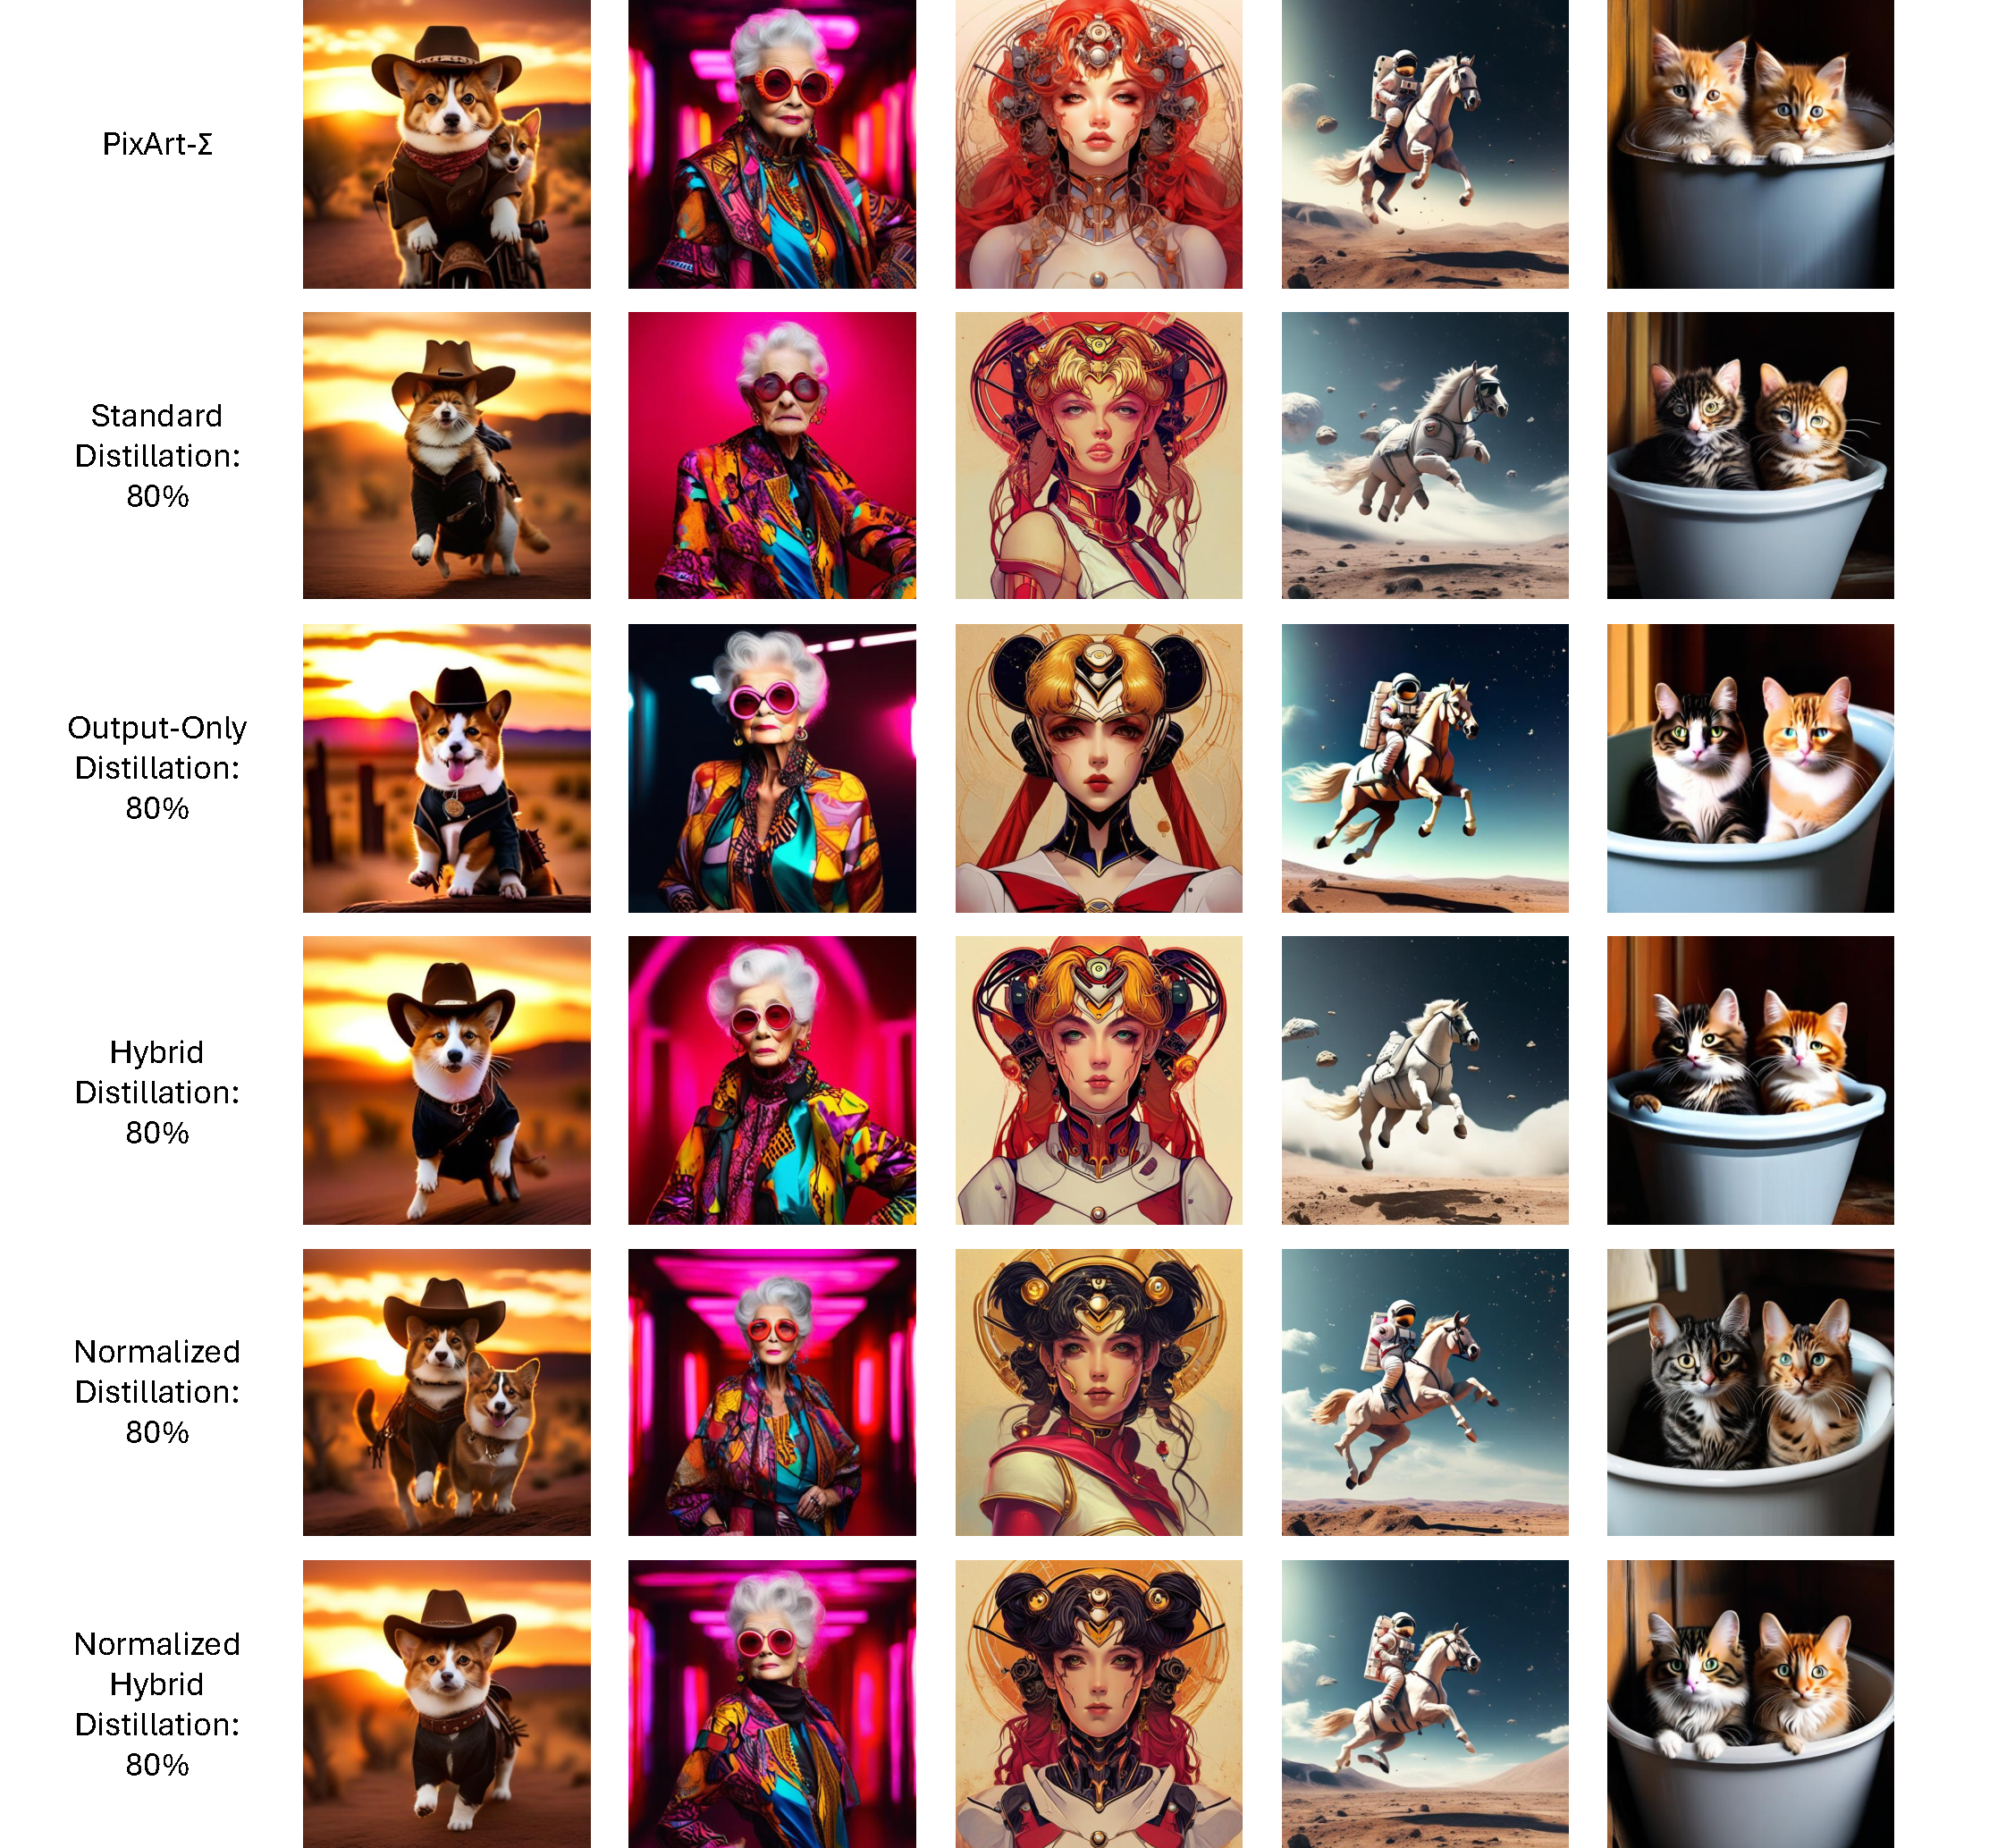
\includegraphics[width=0.65\textwidth]{images/Appendix/KnowledgeDistillation/model_80.pdf}
	\caption[Qualitative Examples: Different Knowledge Distillation Loss Configurations (80\% Model)]{Qualitative comparison of example images generated by models compressed to 80\% using various knowledge distillation loss configurations}
	\label{fig:QualitativeLossInvestigation_80}
\end{figure}

\begin{figure}[H]
	\centering
	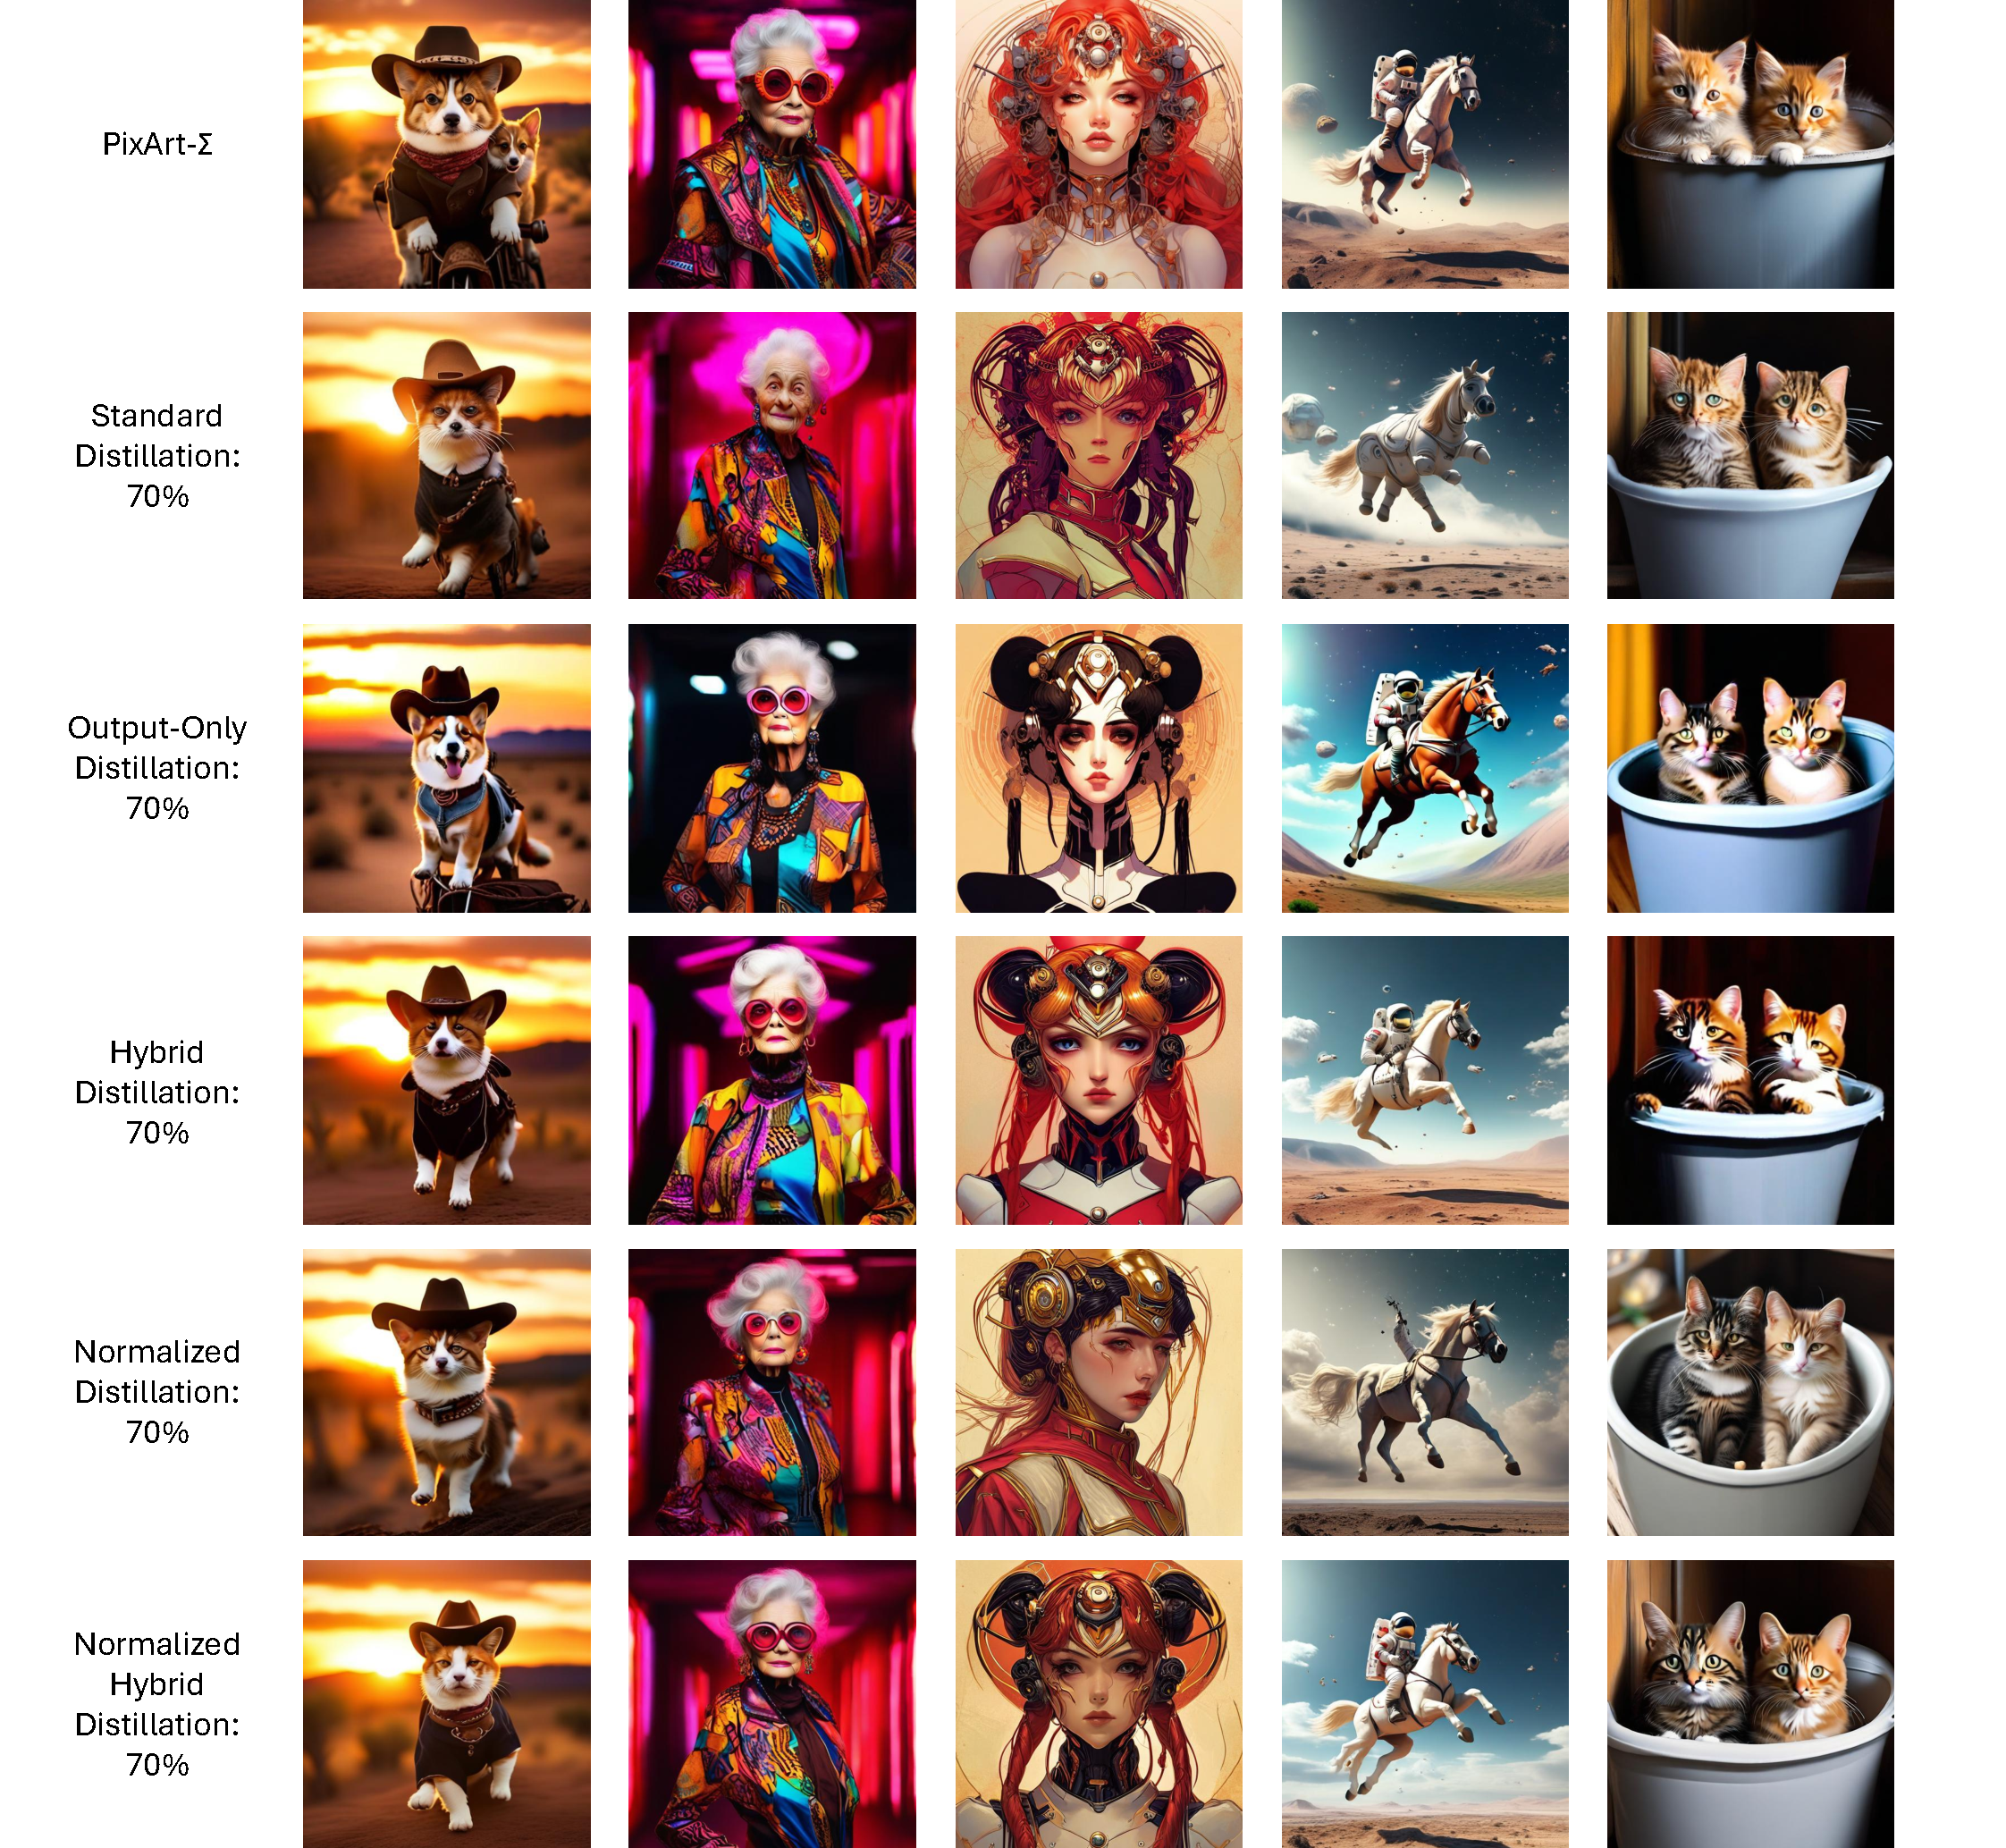
\includegraphics[width=0.65\textwidth]{images/Appendix/KnowledgeDistillation/model_70.pdf}
	\caption[Qualitative Examples: Different Knowledge Distillation Loss Configurations (70\% Model)]{Qualitative comparison of example images generated by models compressed to 70\% using various knowledge distillation loss configurations}
	\label{fig:QualitativeLossInvestigation_70}
\end{figure}

\begin{figure}[H]
	\centering
	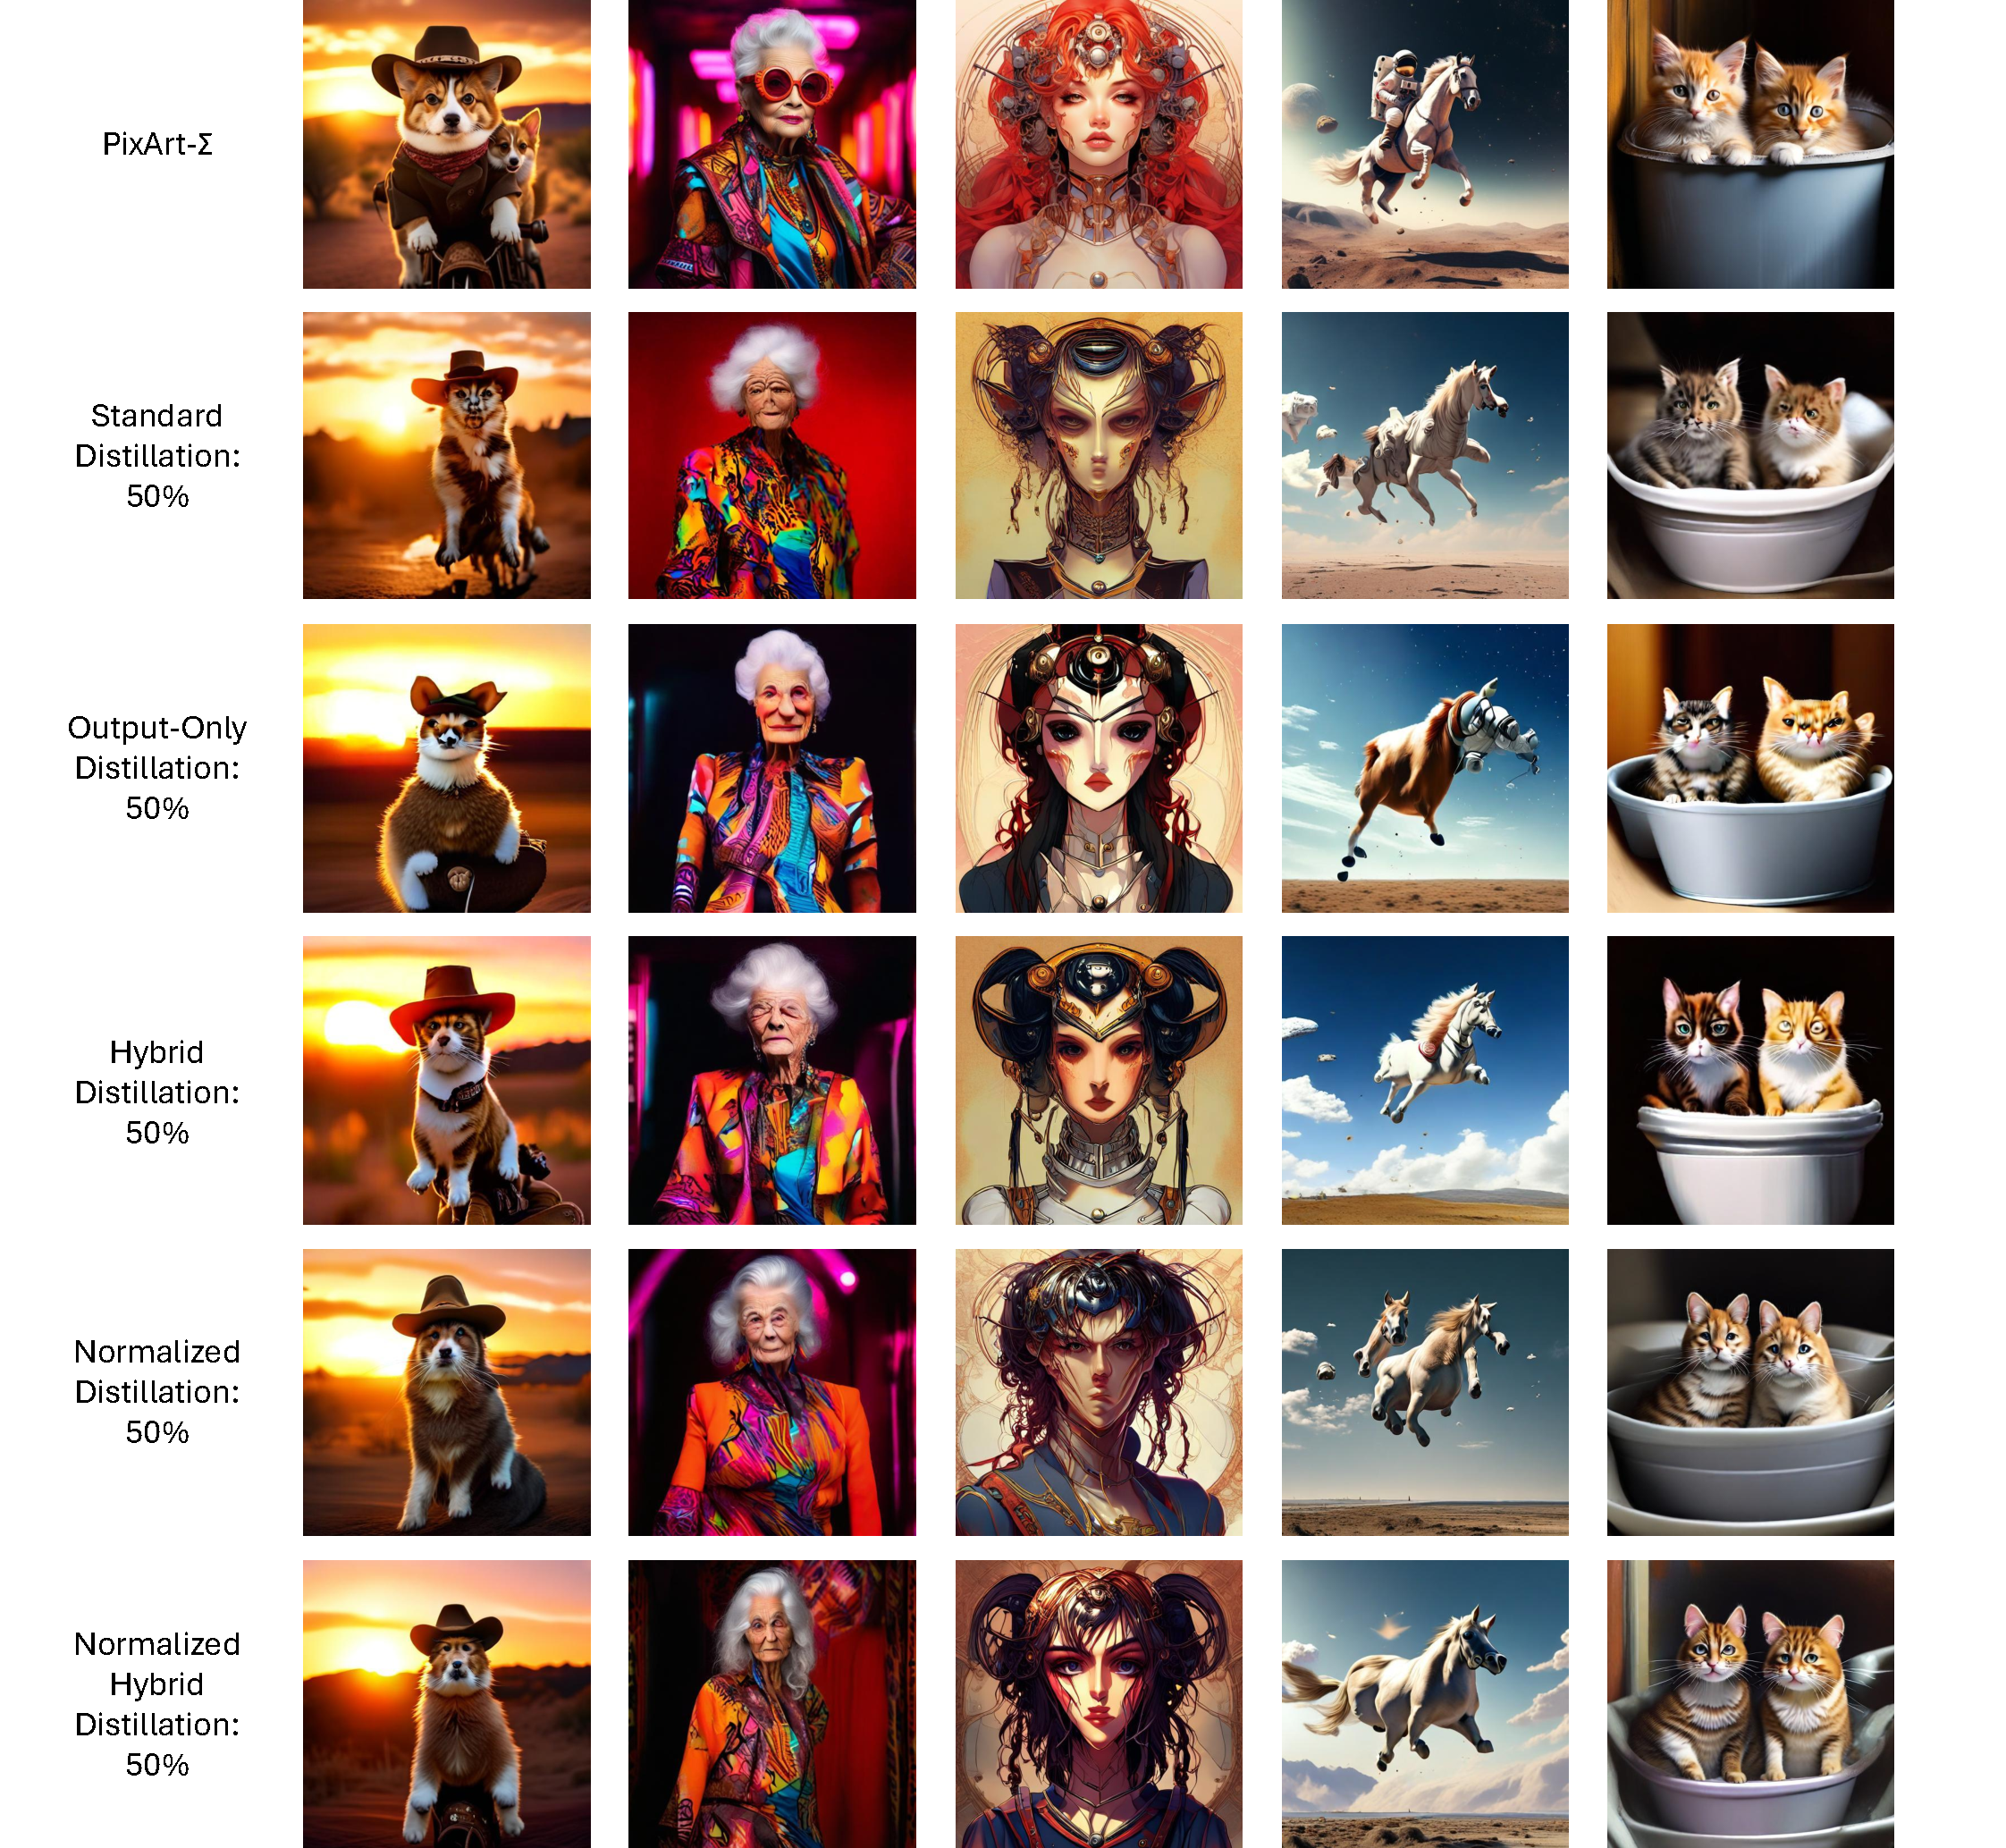
\includegraphics[width=0.65\textwidth]{images/Appendix/KnowledgeDistillation/model_50.pdf}
	\caption[Qualitative Examples: Different Knowledge Distillation Loss Configurations (50\% Model)]{Qualitative comparison of example images generated by models compressed to 50\% using various knowledge distillation loss configurations}
	\label{fig:QualitativeLossInvestigation_50}
\end{figure}



\section{Fine-Tuning Protocol}
\label{sec:FinetuningProtocolAppendix}
This section presents qualitative examples of the three fine-tuning protocols for PixArt-$\Sigma$ (Sec. \ref{sec:fine-tuningProtocol}) compressed to various sizes (Figs. \ref{fig:FinetuningProtocol_90} - \ref{fig:AppxFinetuningProtocol_50}).

\begin{figure}[H]
	\centering
	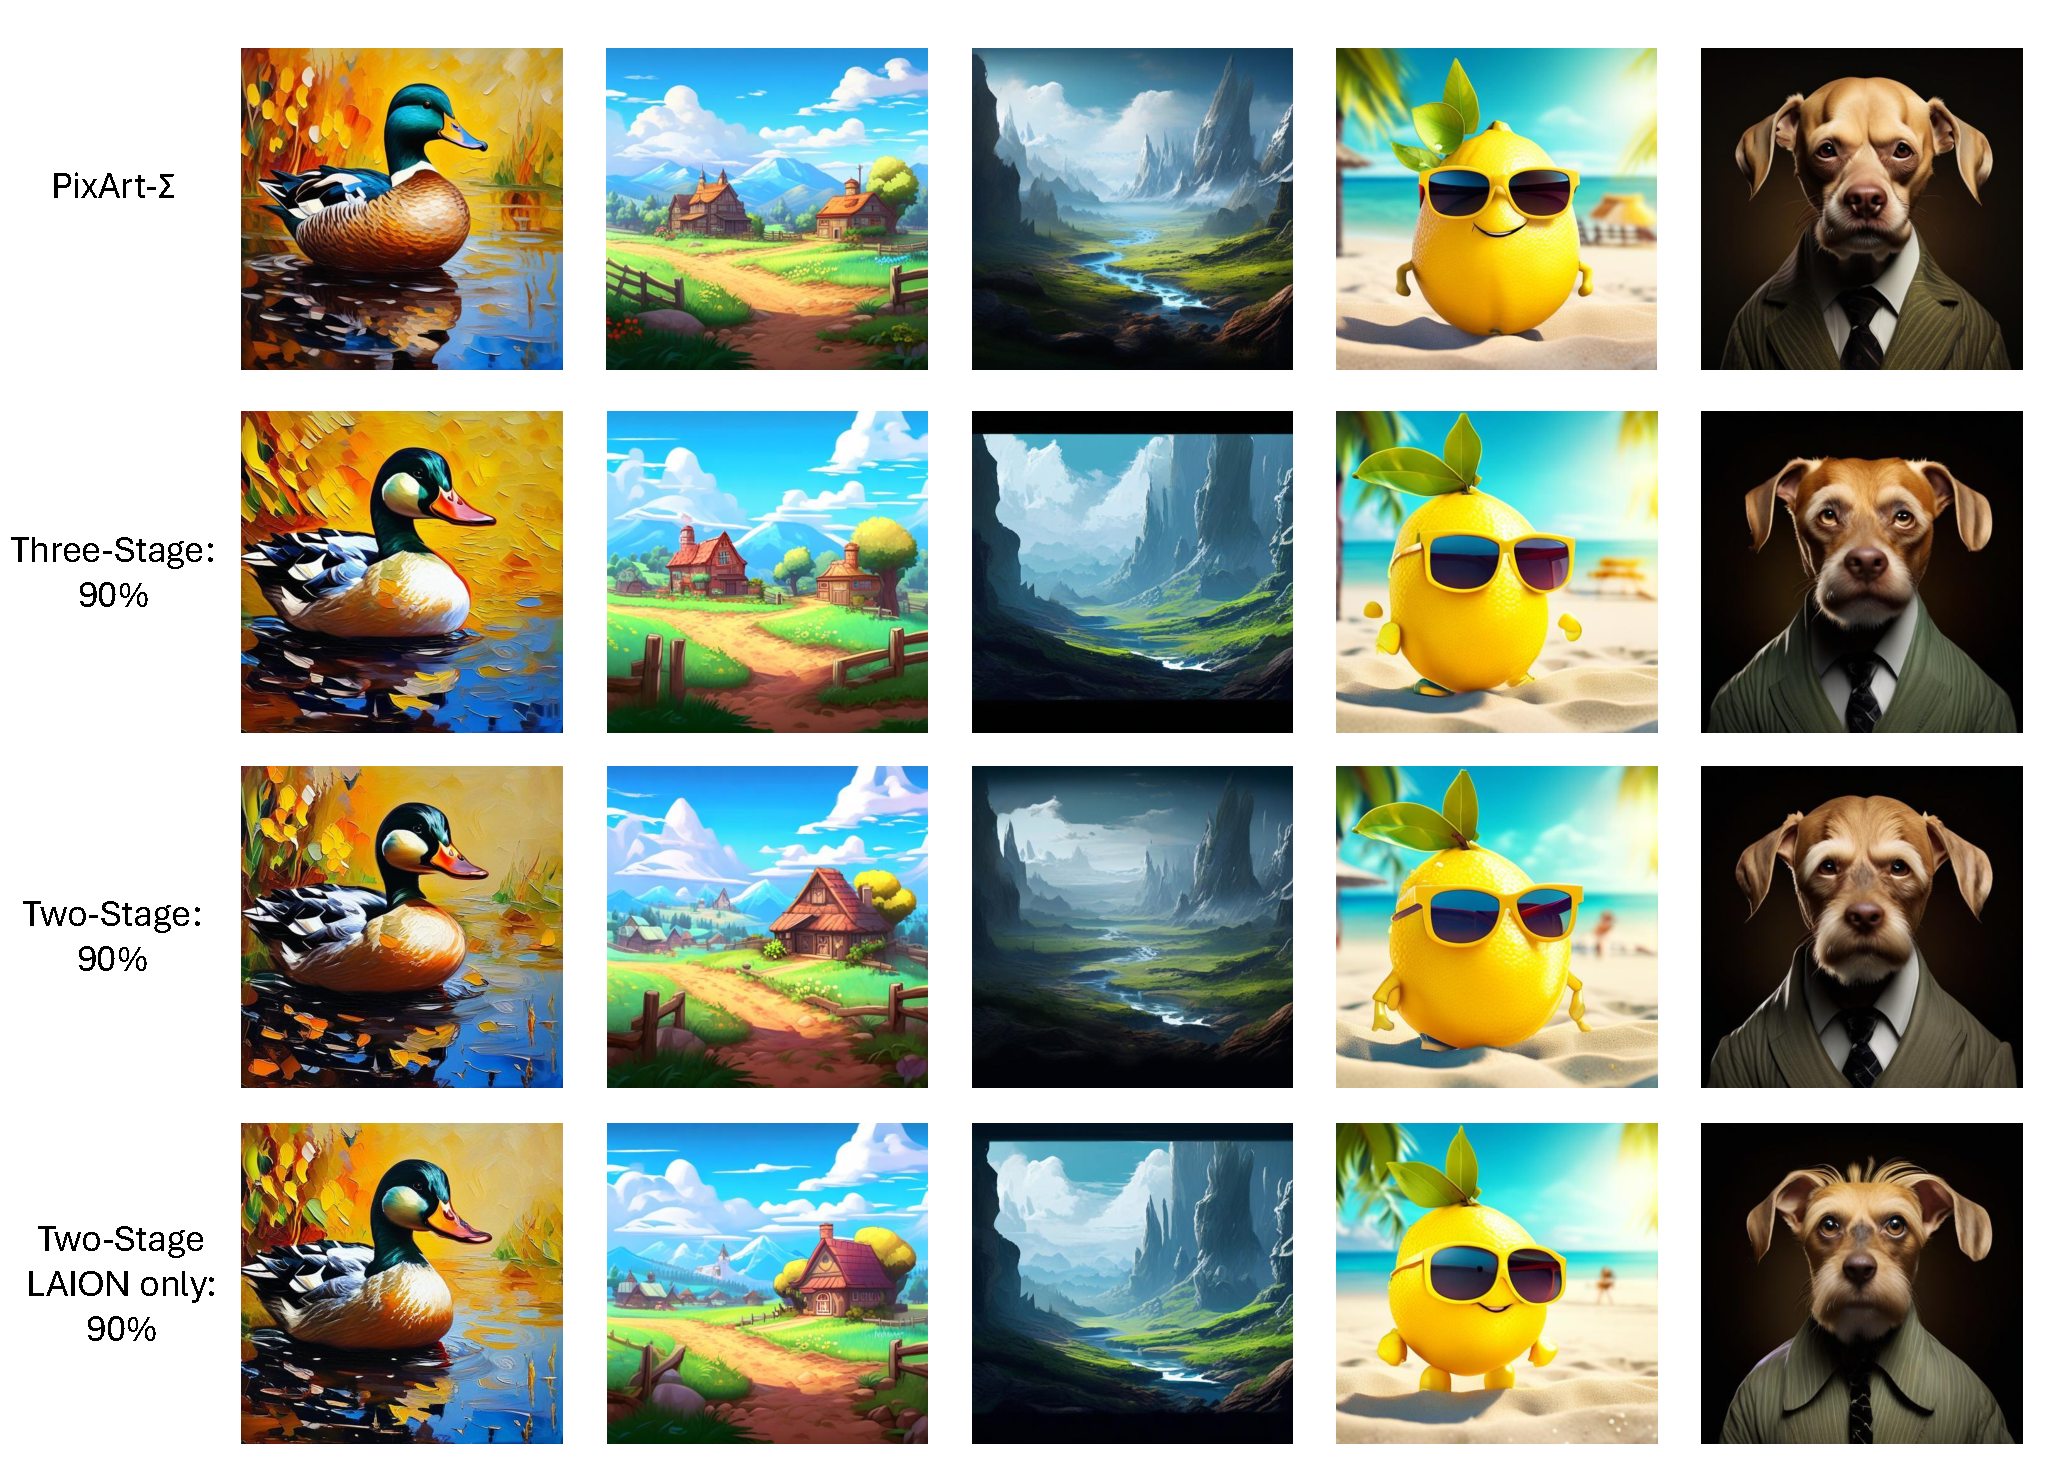
\includegraphics[width=0.7\textwidth]{images/Appendix/FinetuningProtocol/model_90.pdf}
	\caption[Qualitative Examples: Fine-Tuning Protocols (90\% Model)]{Qualitative comparison of example images generated by models compressed to 90\% using various fine-tuning protocols.}
	\label{fig:FinetuningProtocol_90}
\end{figure}

\begin{figure}[H]
	\centering
	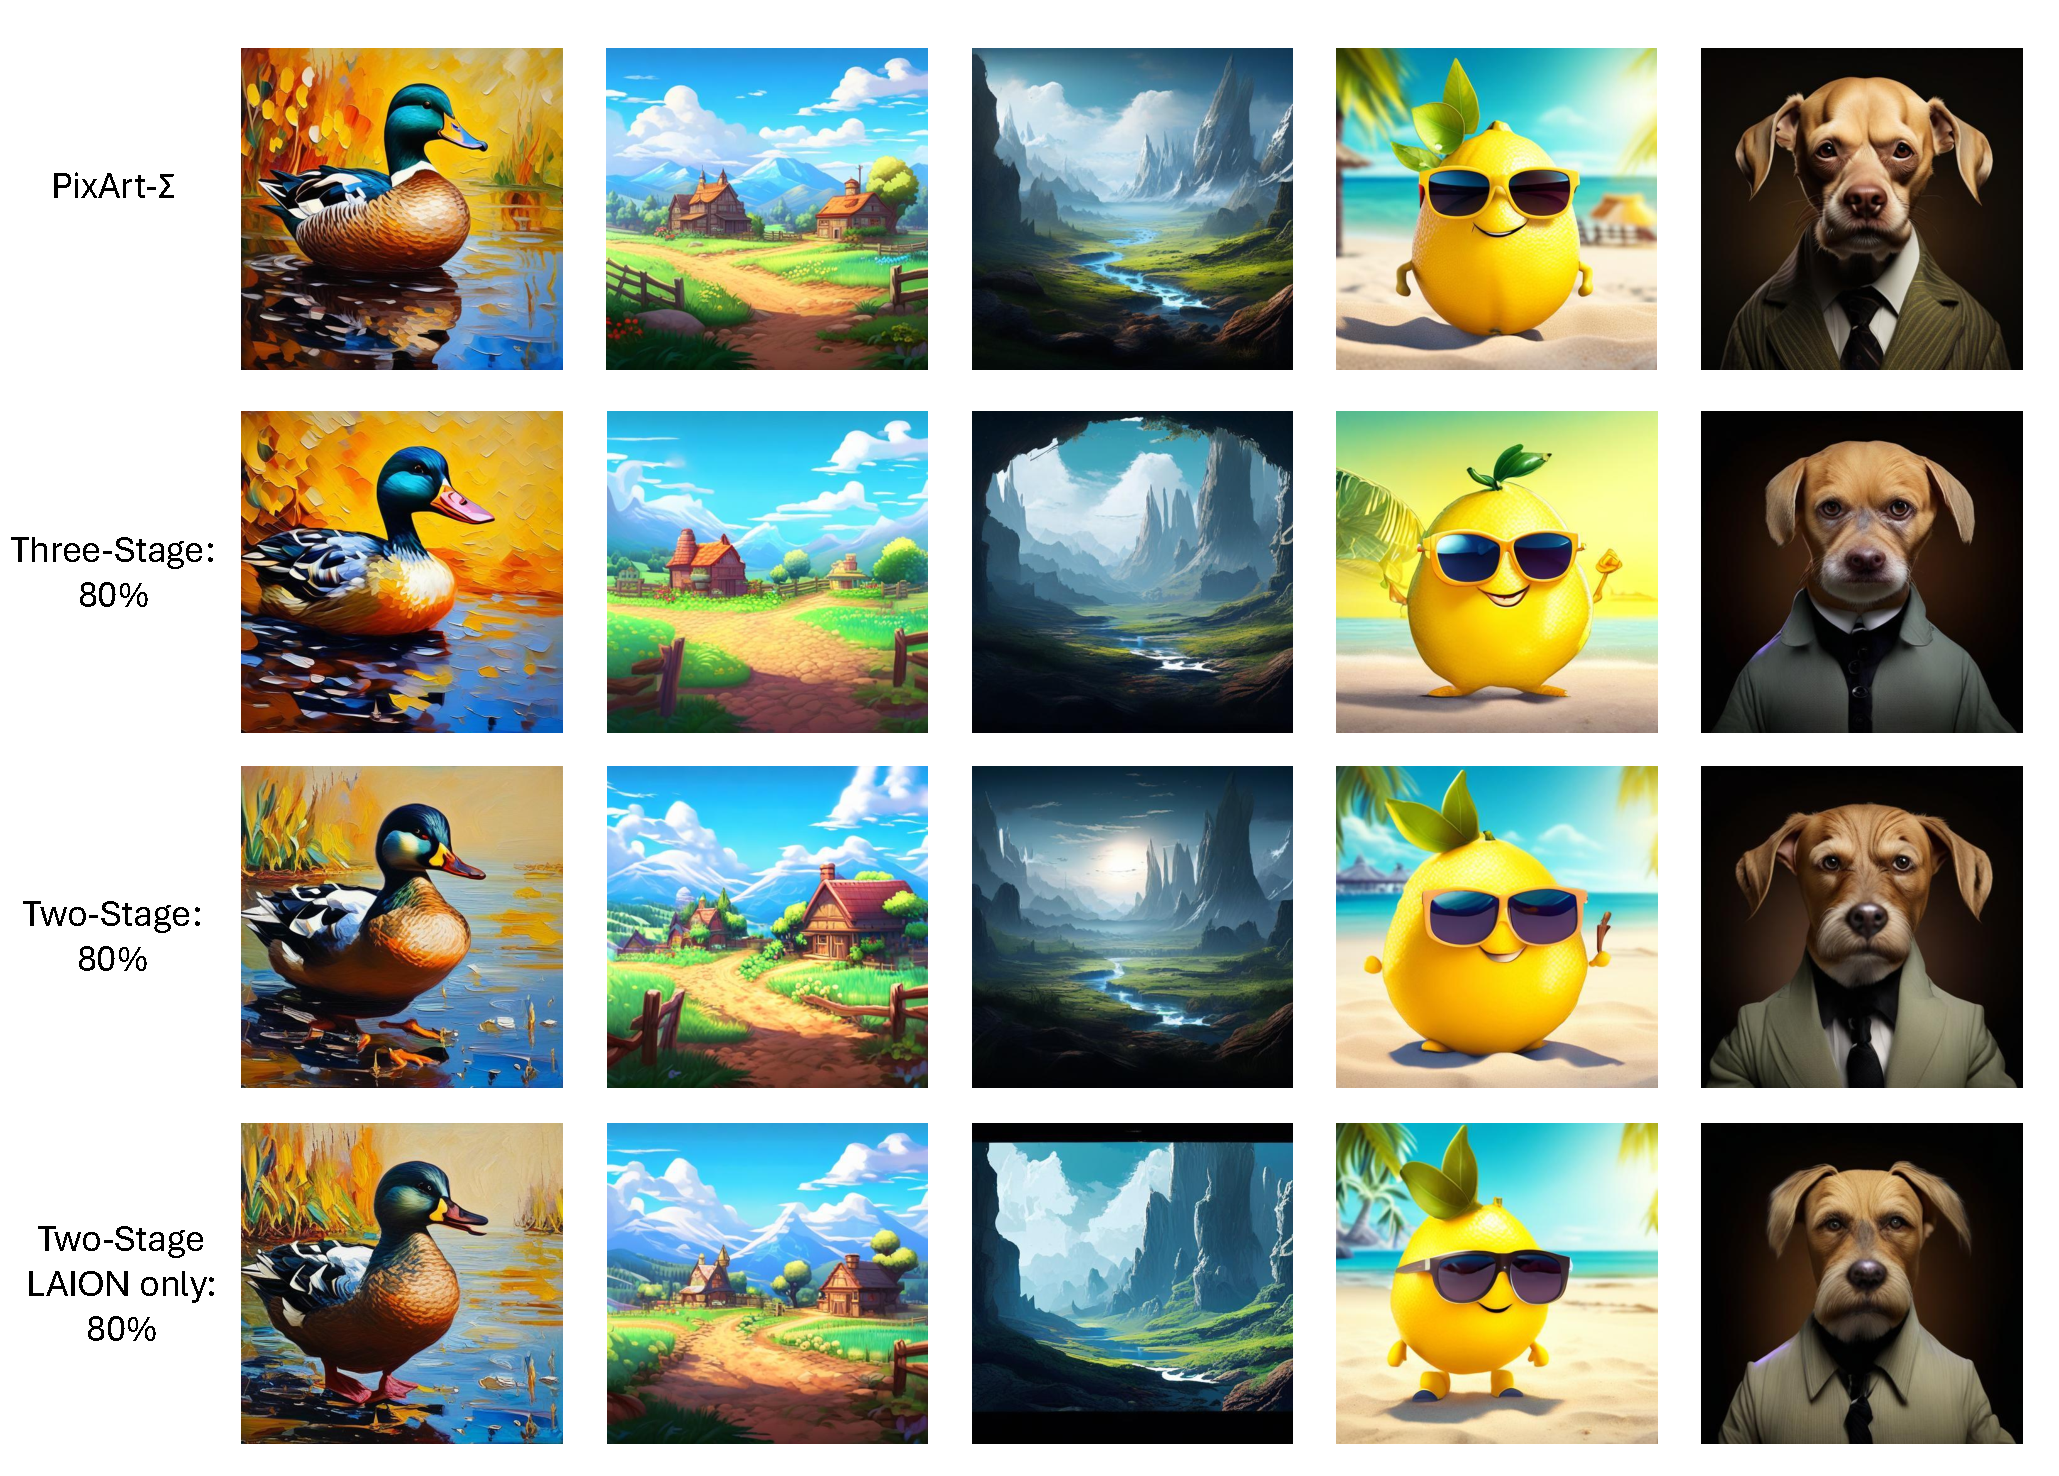
\includegraphics[width=0.7\textwidth]{images/Appendix/FinetuningProtocol/model_80.pdf}
	\caption[Qualitative Examples: Fine-Tuning Protocols (80\% Model)]{Qualitative comparison of example images generated by models compressed to 80\% using various fine-tuning protocols.}
	\label{fig:AppxFinetuningProtocol_80}
\end{figure}

\begin{figure}[H]
	\centering
	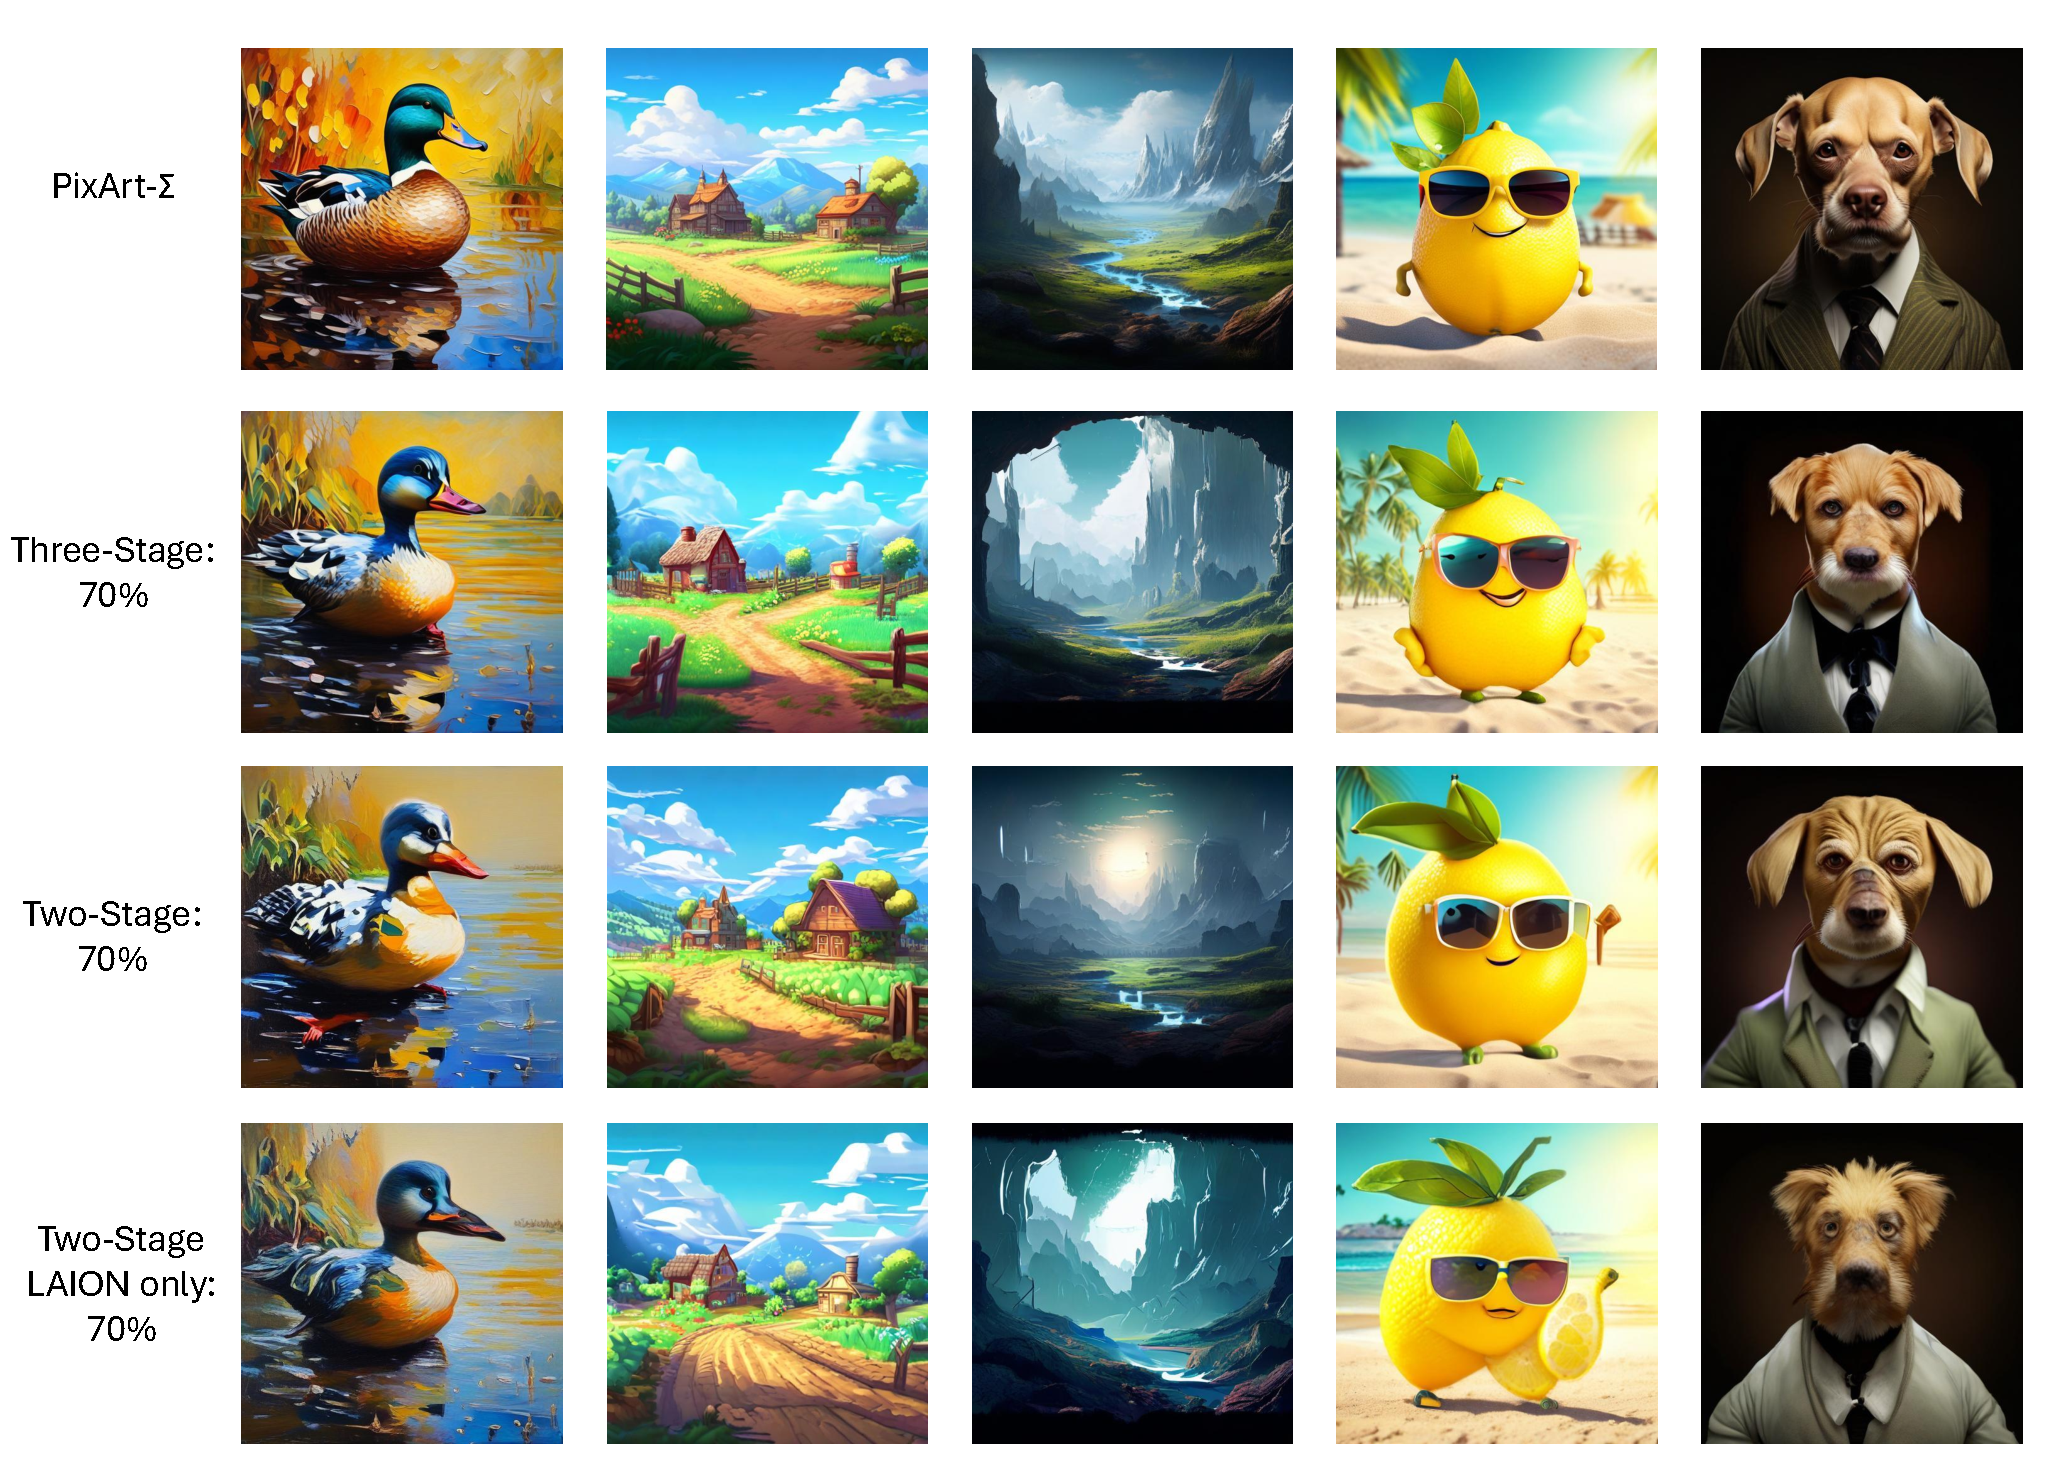
\includegraphics[width=0.7\textwidth]{images/Appendix/FinetuningProtocol/model_70.pdf}
	\caption[Qualitative Examples: Fine-Tuning Protocols (70\% Model)]{Qualitative comparison of example images generated by models compressed to 70\% using various fine-tuning protocols.}
	\label{fig:AppxFinetuningProtocol_70}
\end{figure}

\begin{figure}[H]
	\centering
	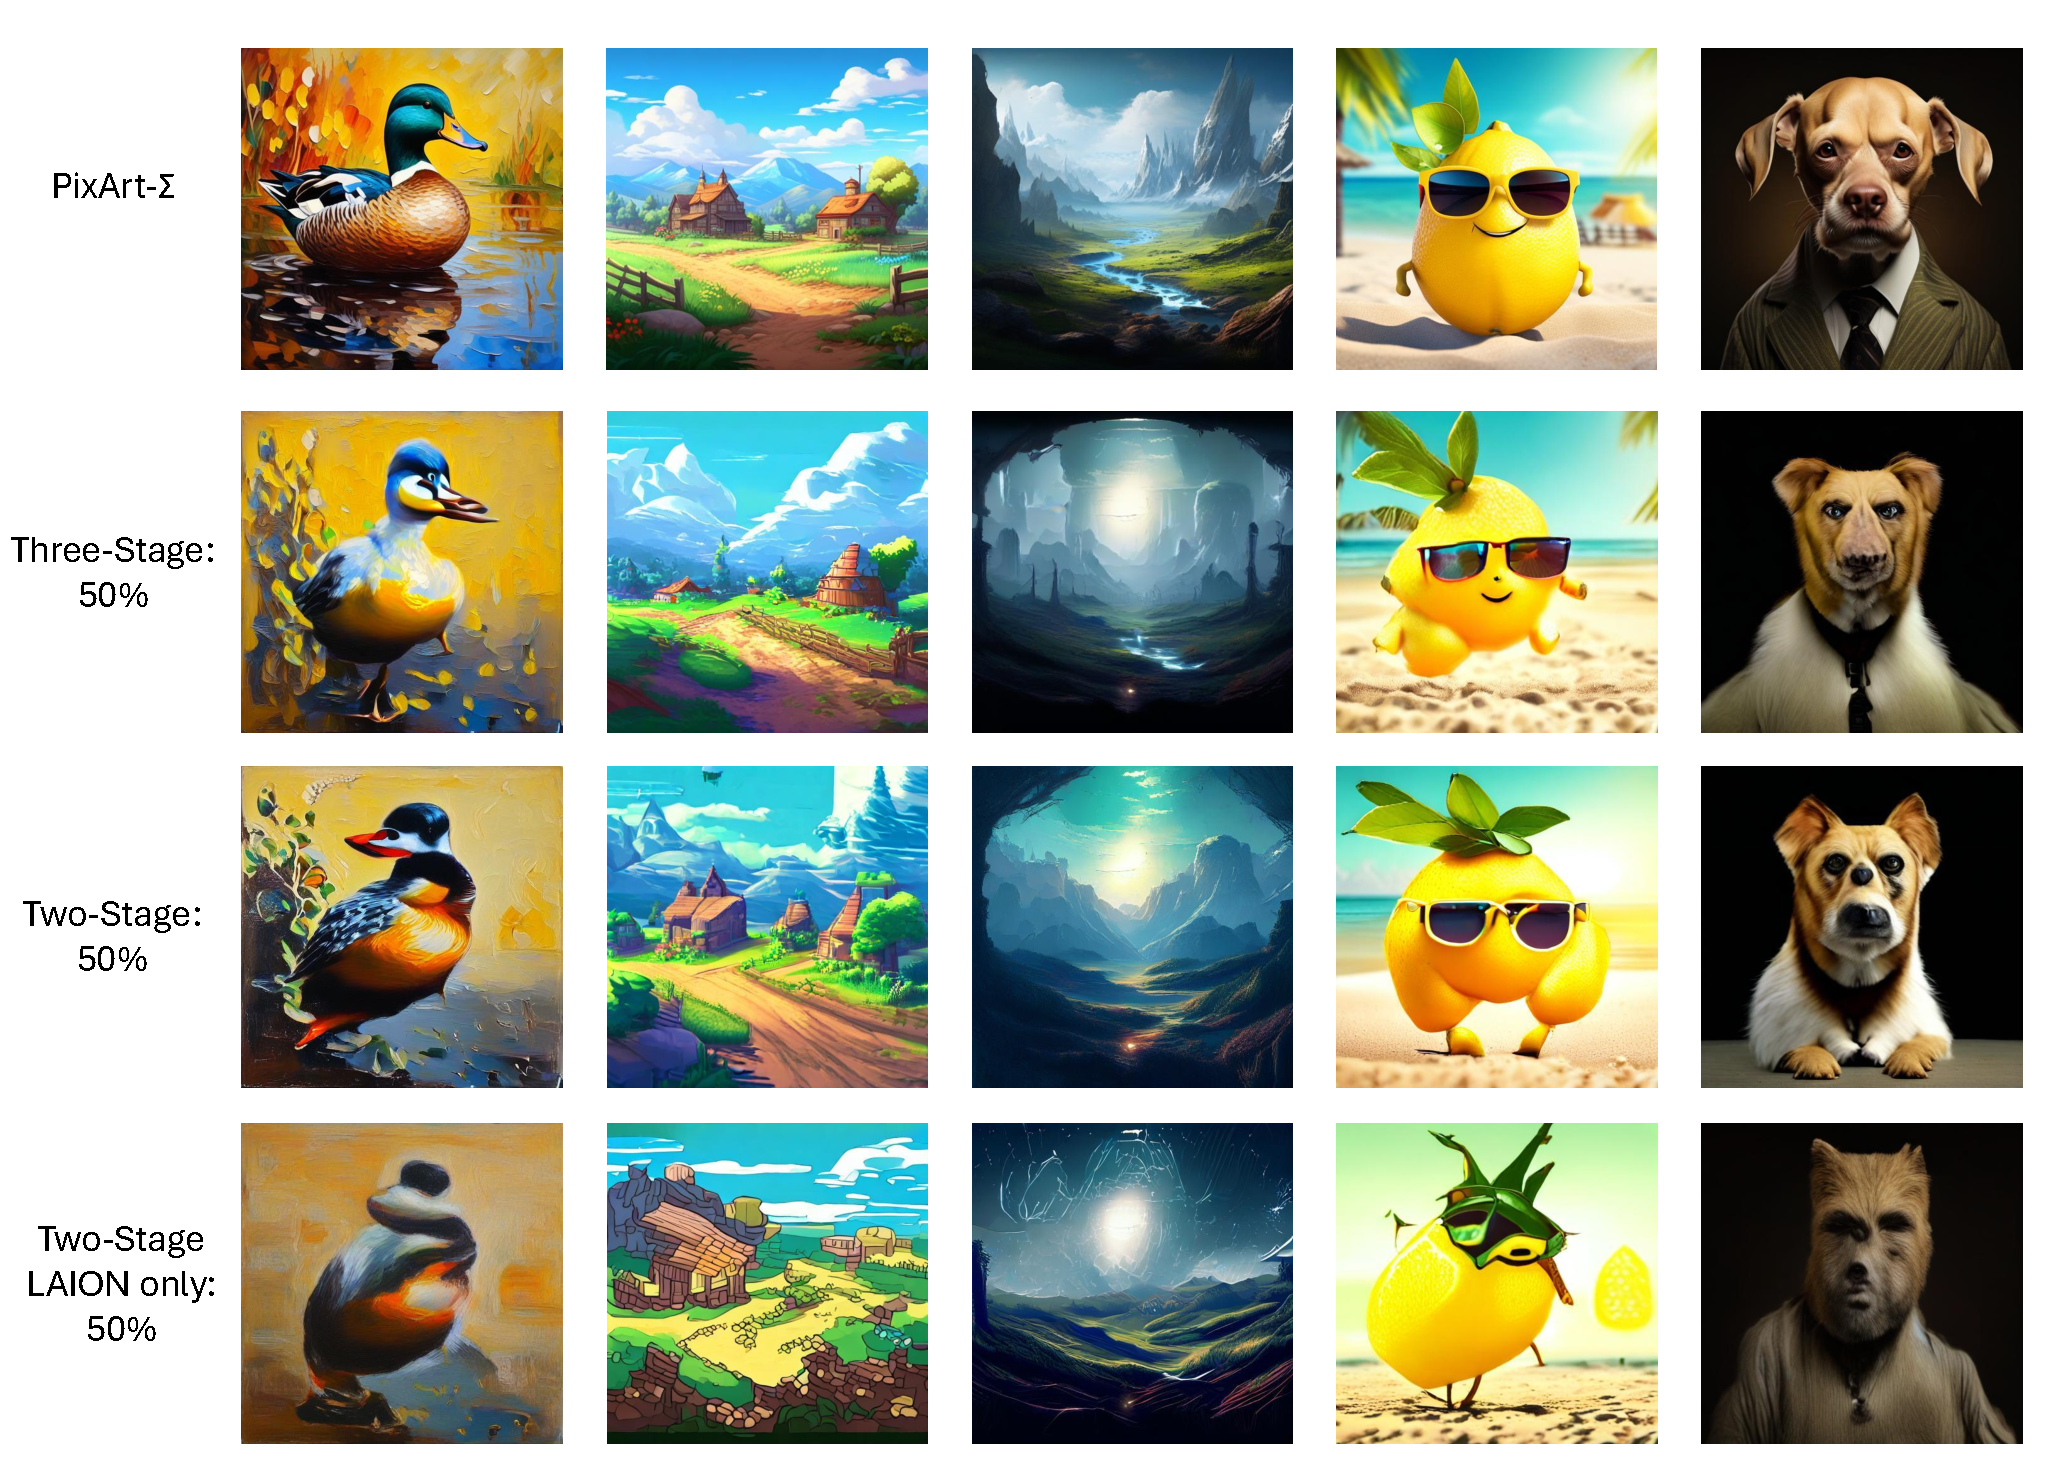
\includegraphics[width=0.7\textwidth]{images/Appendix/FinetuningProtocol/model_50.pdf}
	\caption[Qualitative Examples: Fine-Tuning Protocols (50\% Model)]{Qualitative comparison of example images generated by models compressed to 50\% using various fine-tuning protocols.}
	\label{fig:AppxFinetuningProtocol_50}
\end{figure}


\section{Compression Strategy}
\label{appx:CompressionStrategy}
In this section, the PixArt-$\Sigma$ architecture is visualized and its components subject to \gls{SVD}-based compression are indicated (Fig. \ref{fig:PixArt_Sigma_Compresseed_Modules_Architecutre}). In addition, it provides qualitative examples comparing \gls{SVD}-based compression with complete block pruning across varying model sizes (Figs. \ref{fig:Example_Images_SVD_vs_Removal_90_Appx} - \ref{fig:Example_Images_SVD_vs_Removal_60_Appx}) complementing the visualization of Sec. \ref{sec:CompressionStrategyPixart}.

\begin{figure}[H]
	\centering
	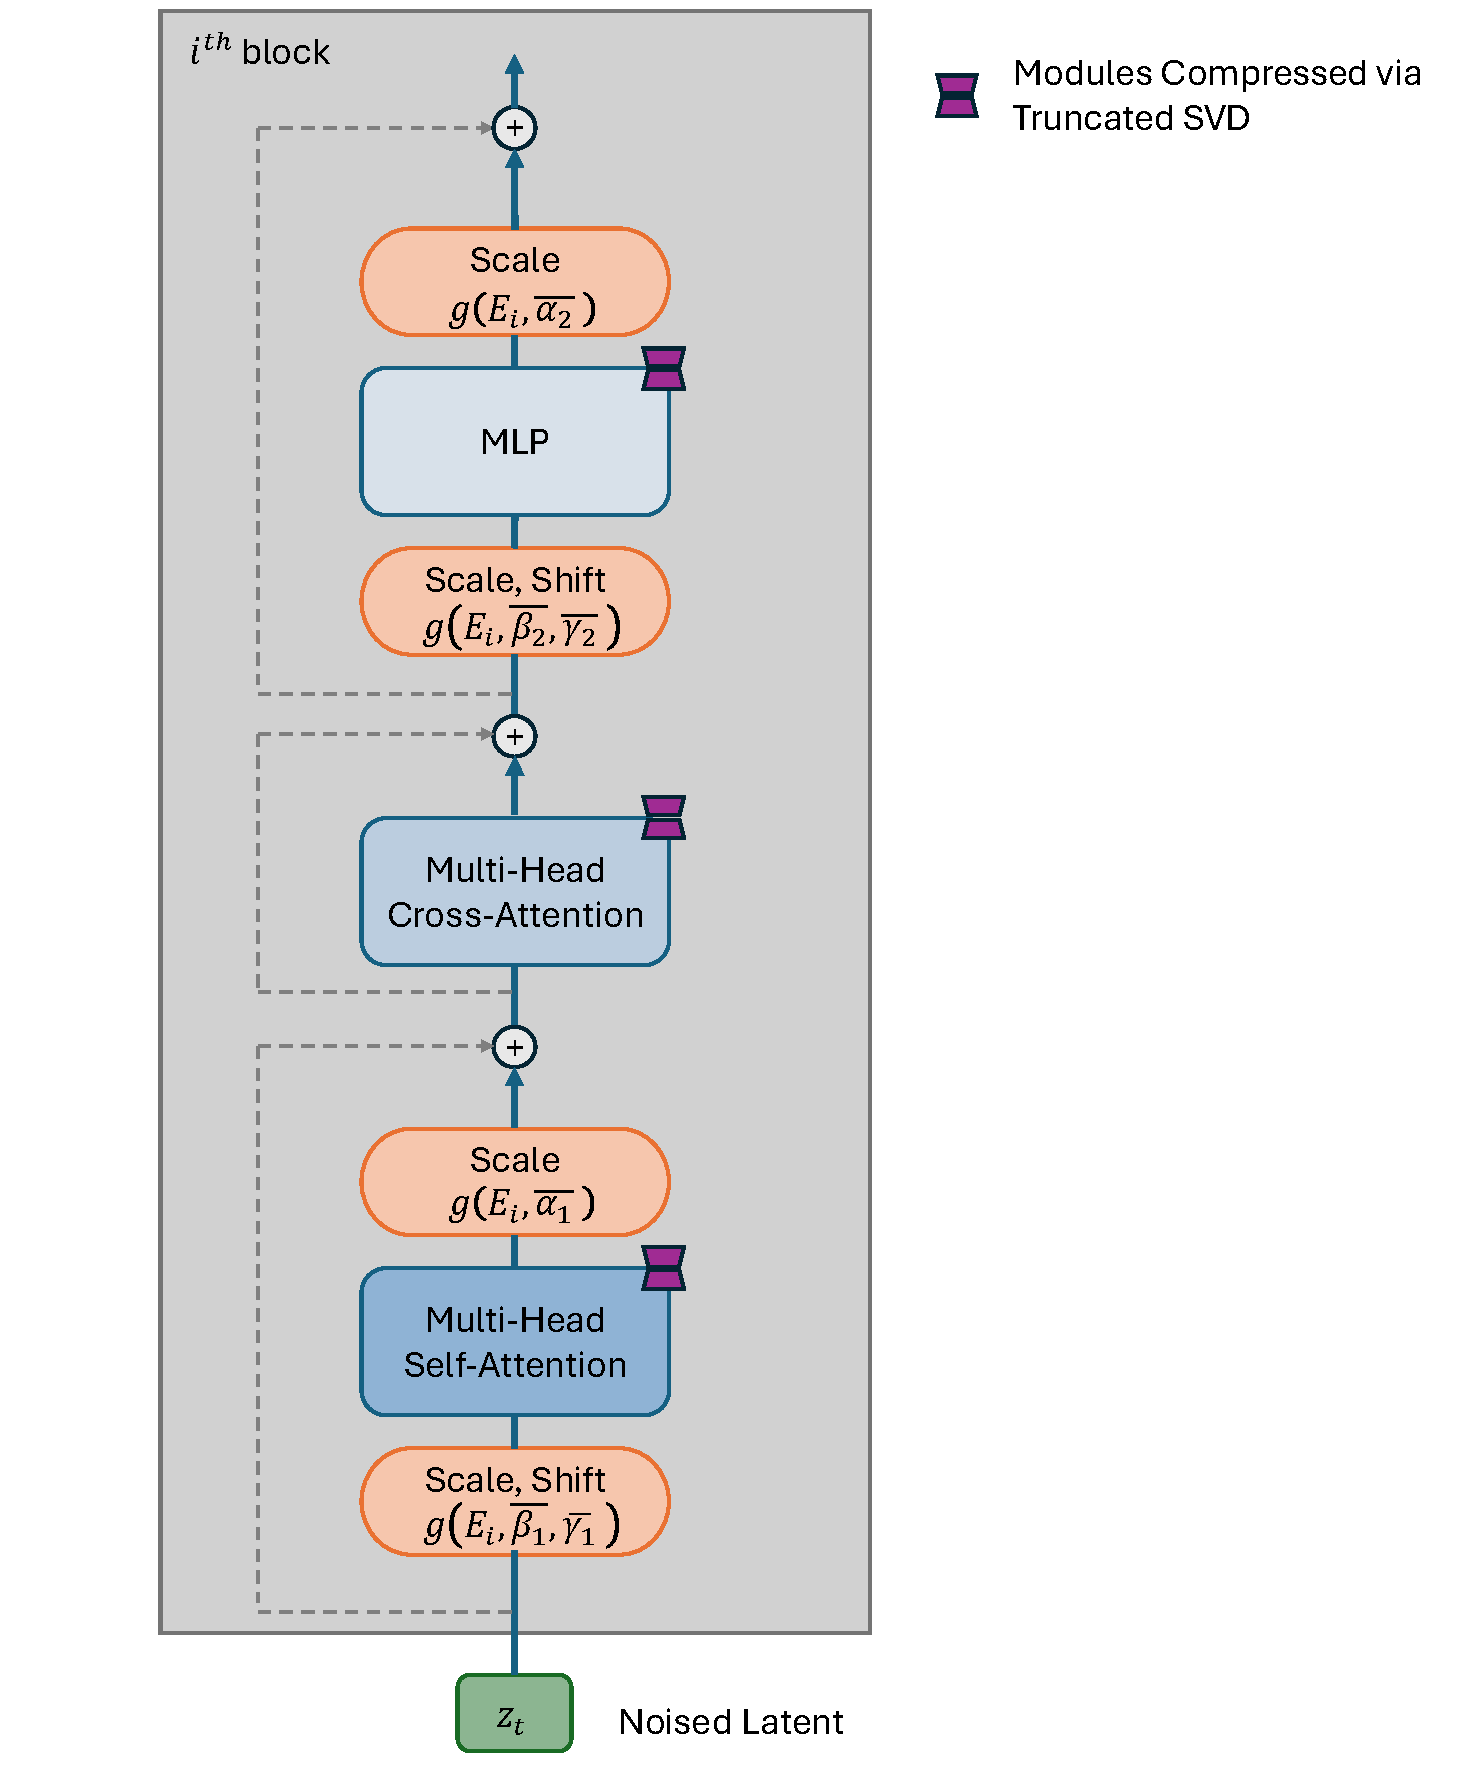
\includegraphics[width=0.5\textwidth]{images/Experimente/SVD_VS_Removal/PixartArchitectureCompressedModules.pdf}
	\caption[\gls{SVD} Compressed Modules within Transformer Blocks of PixArt-$\Sigma$]{\gls{SVD} Compressed Modules within Transformer Blocks of PixArt-$\Sigma$.}
	\label{fig:PixArt_Sigma_Compresseed_Modules_Architecutre}
\end{figure}

\begin{figure}[H]
	\centering
	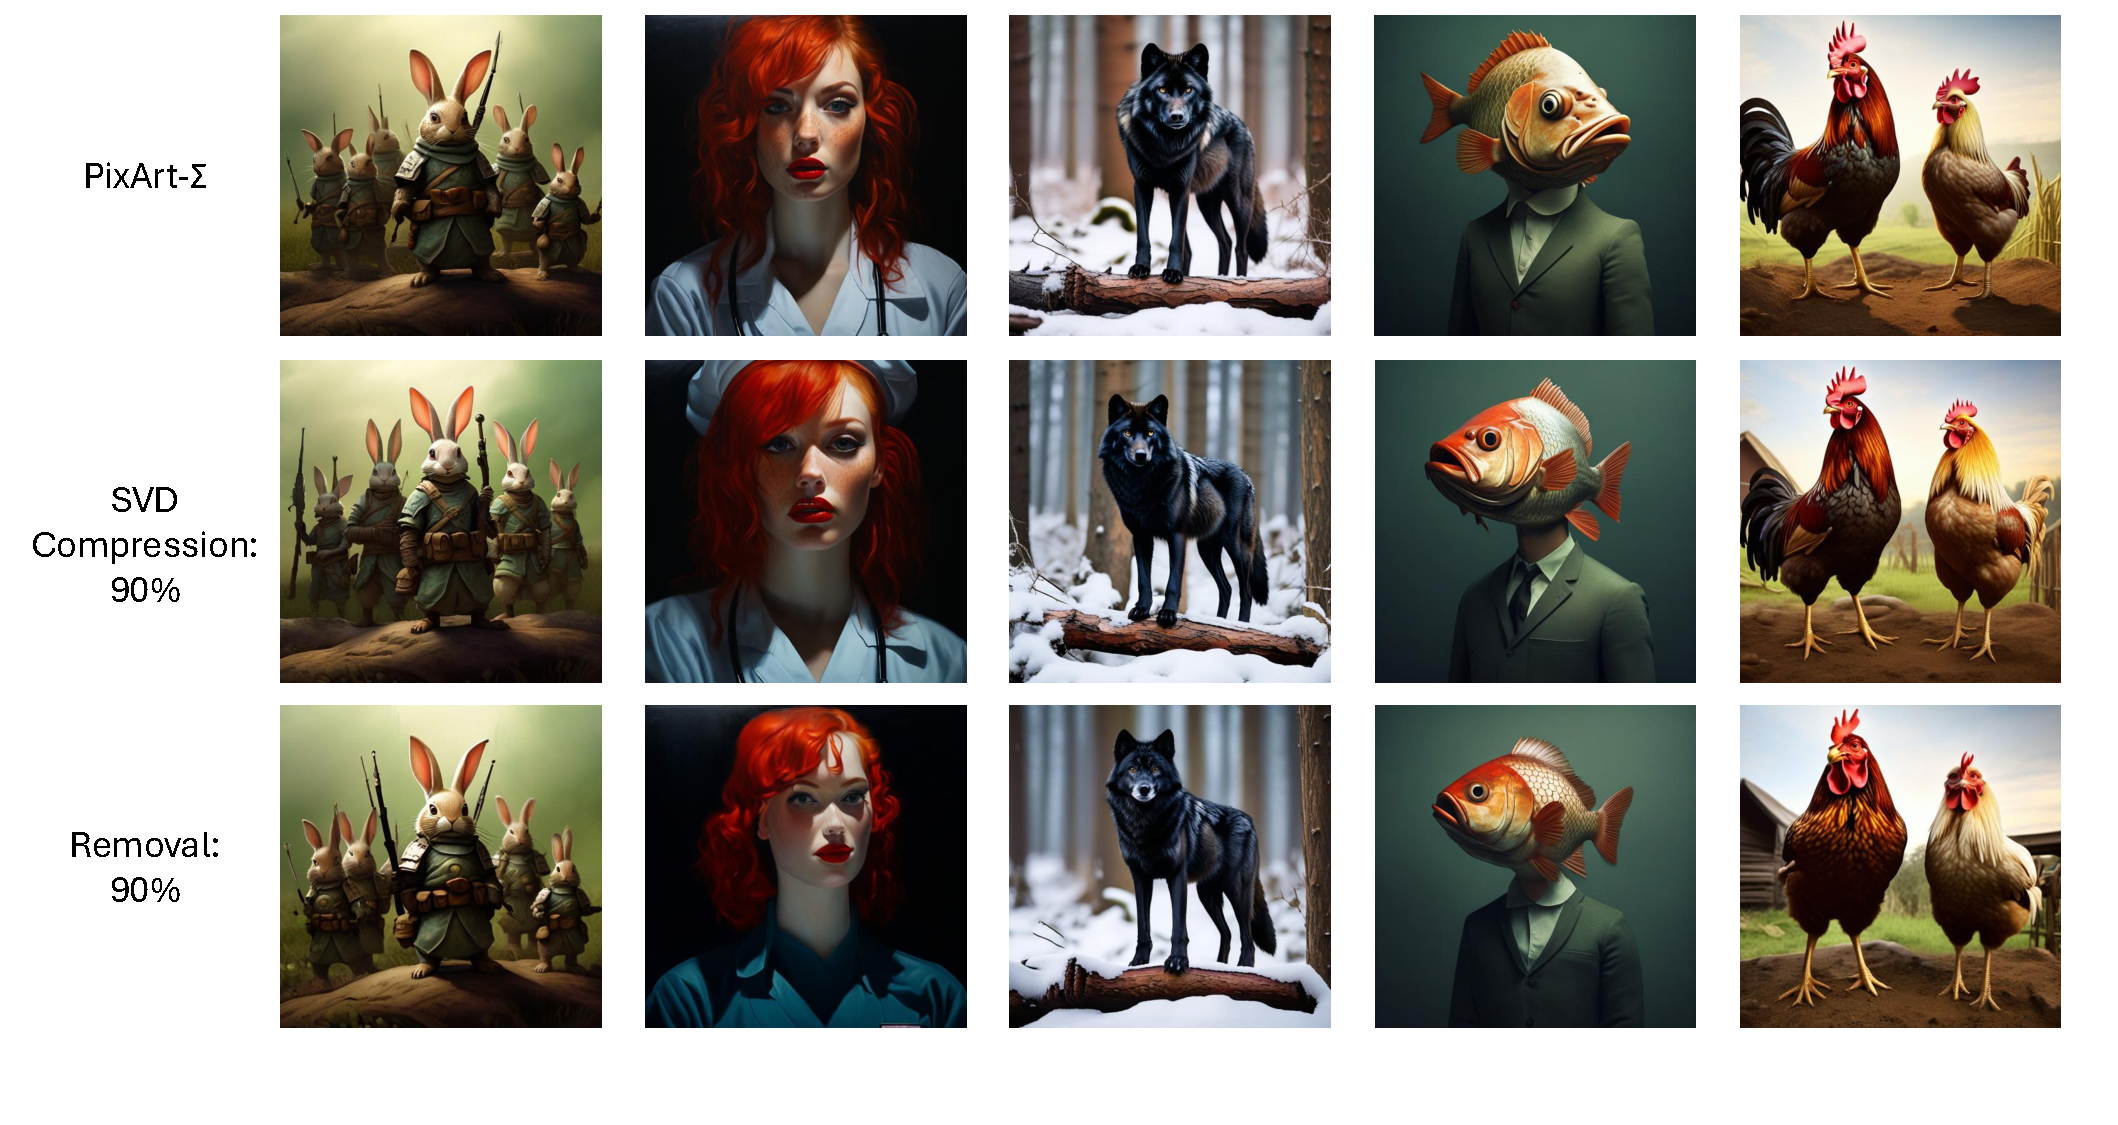
\includegraphics[width=0.9\textwidth]{images/Experimente/SVD_VS_Removal/ImageExamples_model90.pdf}
	\caption[Qualitative Examples: Compression Strategies (90\% Model)]{Qualitative comparison of example images generated by models compressed to 90\% using complete block pruning versus \gls{SVD}-based block compression.}
	\label{fig:Example_Images_SVD_vs_Removal_90_Appx}
\end{figure}

\begin{figure}[H]
	\centering
	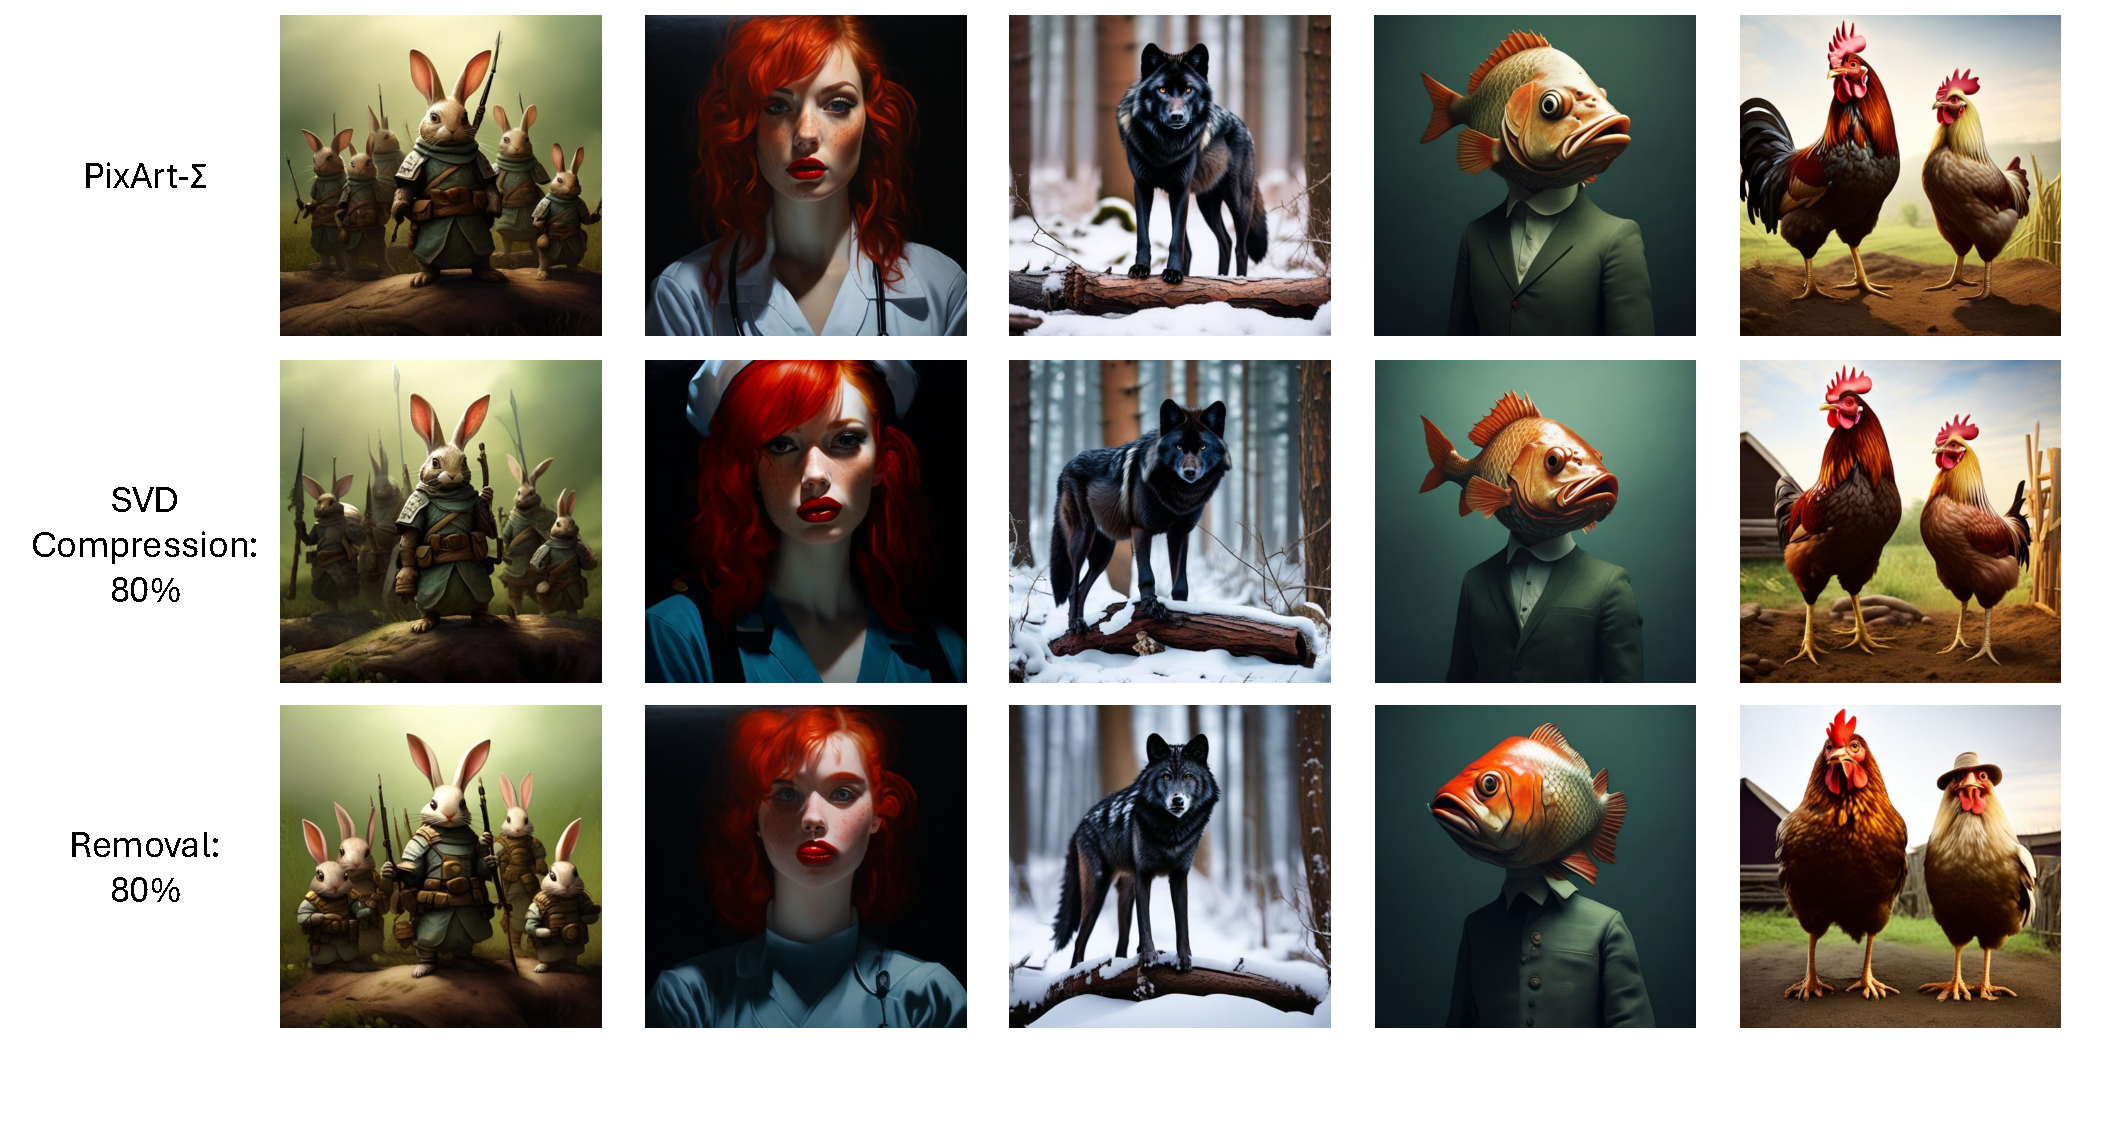
\includegraphics[width=0.9\textwidth]{images/Experimente/SVD_VS_Removal/ImageExamples_model80.pdf}
	\caption[Qualitative Examples: Compression Strategies (80\% Model)]{Qualitative comparison of example images generated by models compressed to 80\% using complete block pruning versus \gls{SVD}-based block compression.}
	\label{fig:Example_Images_SVD_vs_Removal_80_Appx}
\end{figure}

\begin{figure}[H]
	\centering
	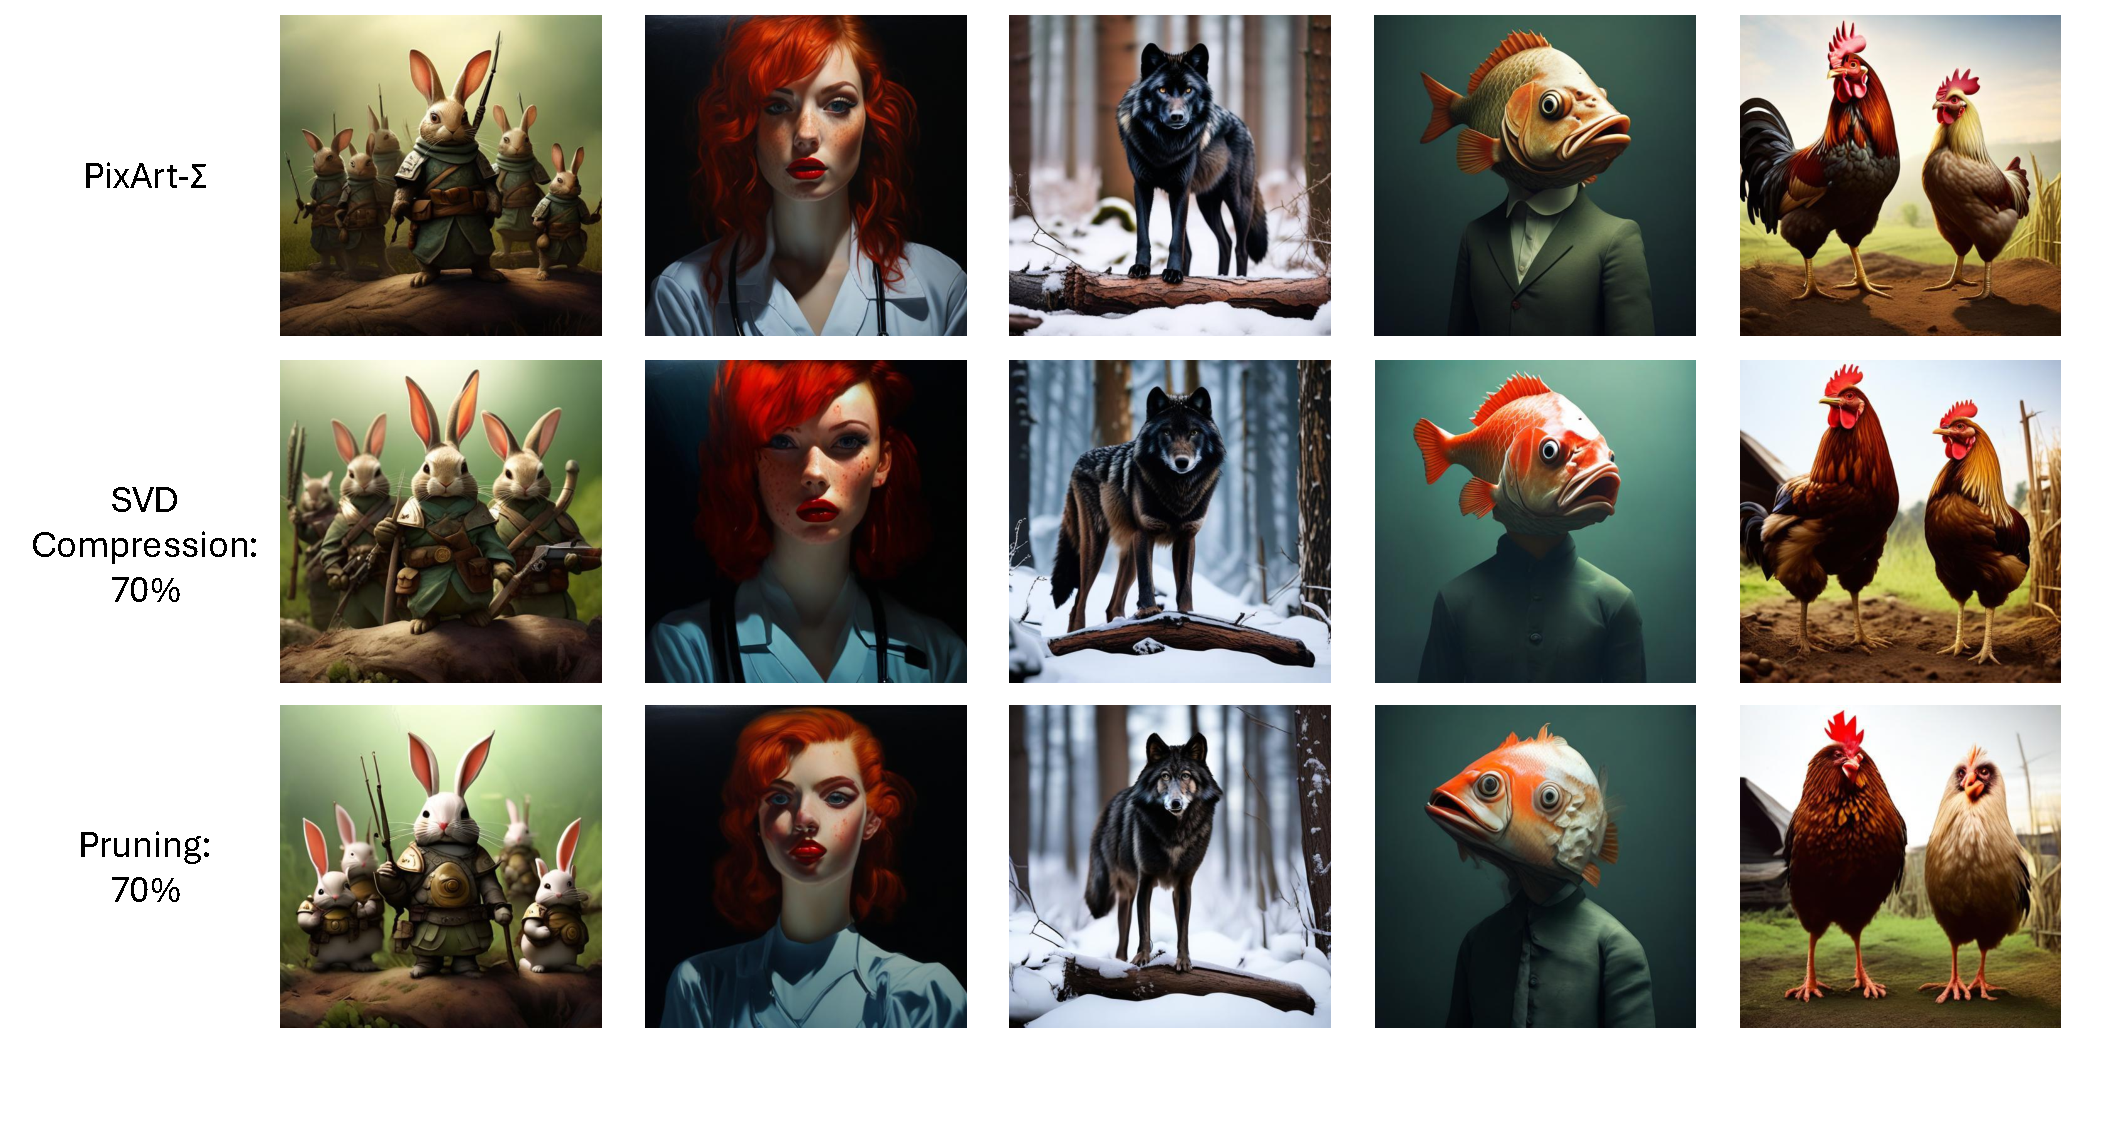
\includegraphics[width=0.9\textwidth]{images/Experimente/SVD_VS_Removal/ImageExamples_model70.pdf}
	\caption[Qualitative Examples: Compression Strategies (70\% Model)]{Qualitative comparison of example images generated by models compressed to 70\% using complete block pruning versus \gls{SVD}-based block compression.}
	\label{fig:Example_Images_SVD_vs_Removal_70_Appx}
\end{figure}

\begin{figure}[H]
	\centering
	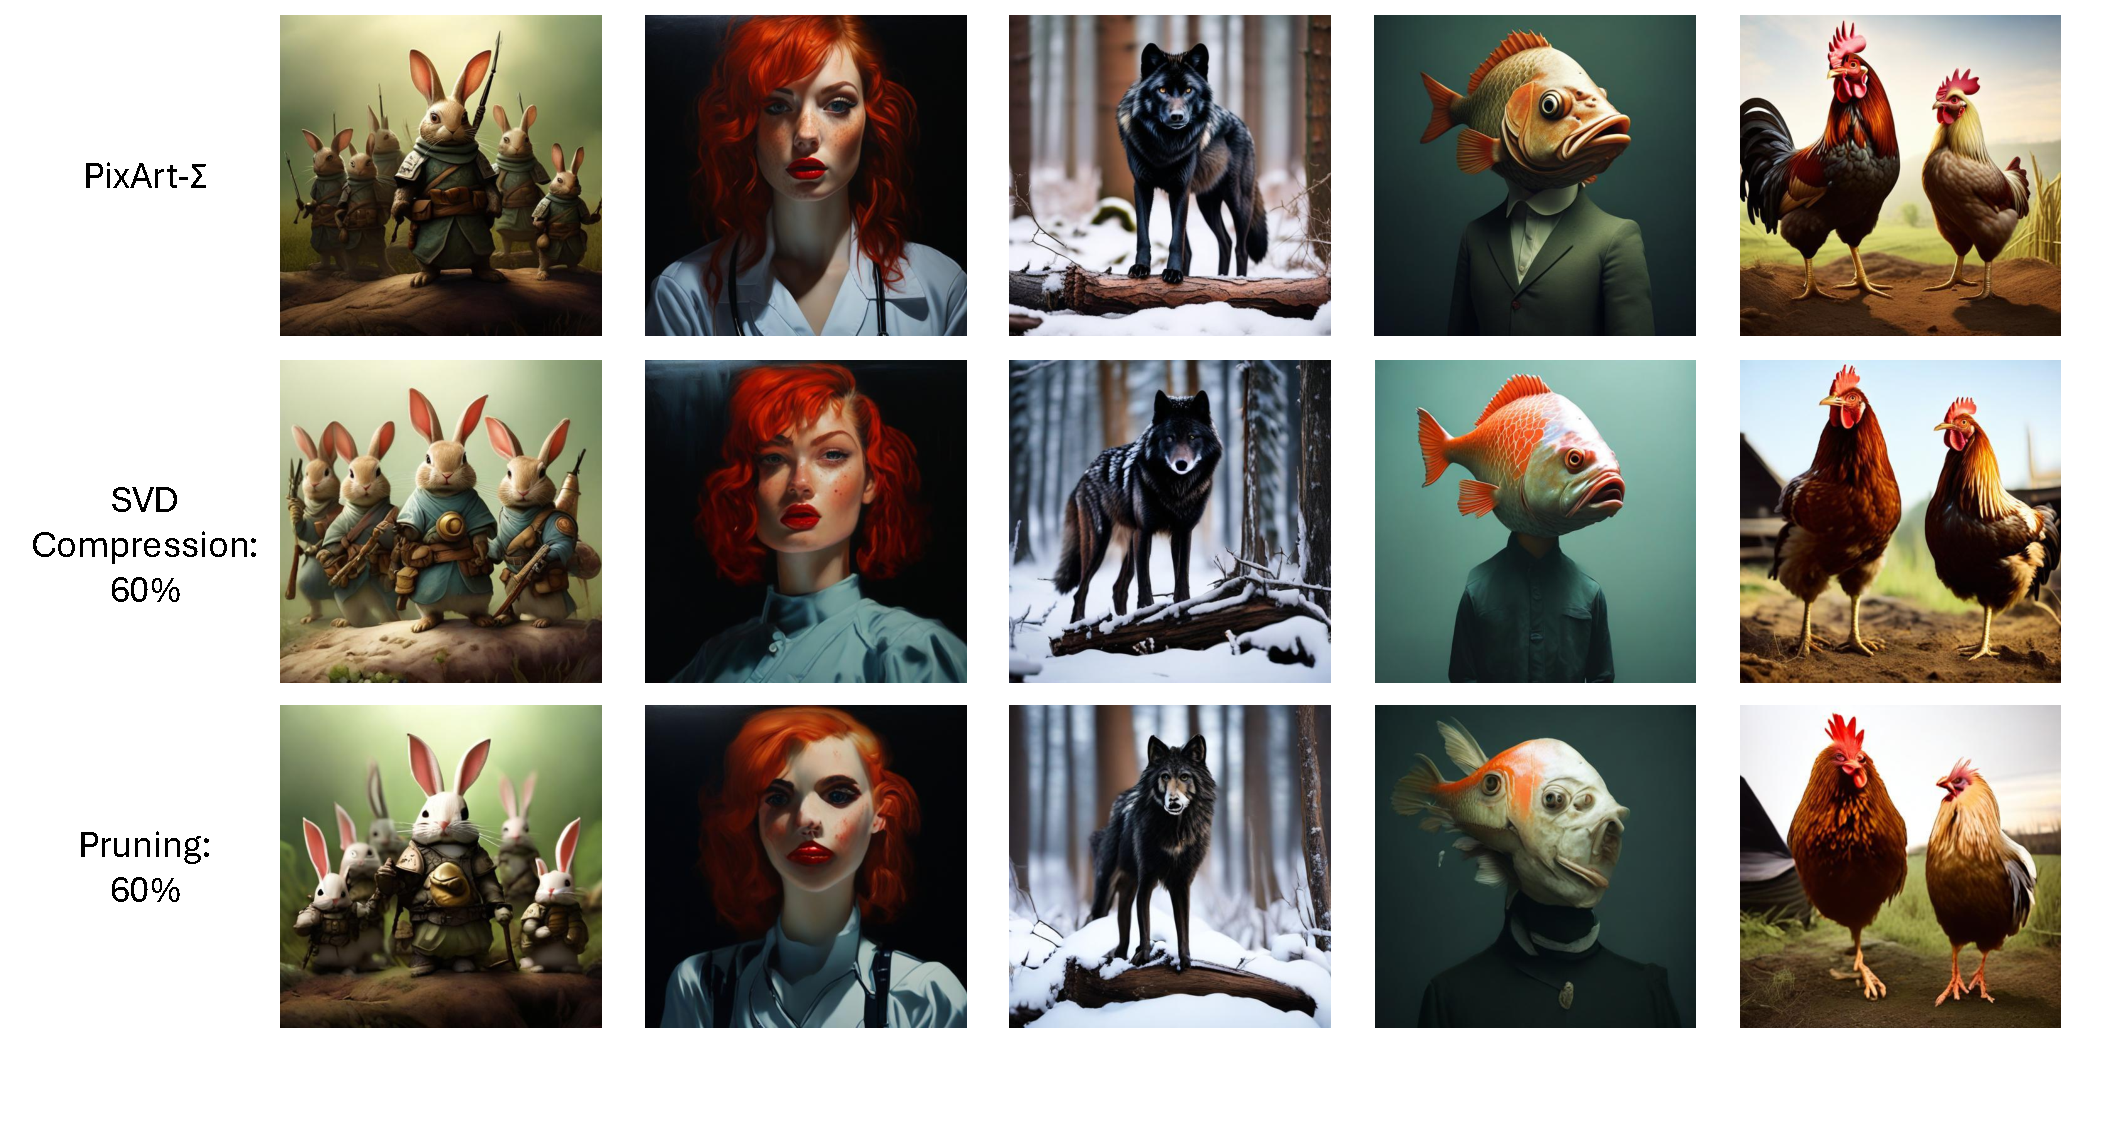
\includegraphics[width=0.9\textwidth]{images/Experimente/SVD_VS_Removal/ImageExamples_model60.pdf}
	\caption[Qualitative Examples: Compression Strategies (60\% Model)]{Qualitative comparison of example images generated by models compressed to 60\% using complete block pruning versus \gls{SVD}-based block compression.}
	\label{fig:Example_Images_SVD_vs_Removal_60_Appx}
\end{figure}



\section{Importance-Aware Rank-Adaptive Progressive Model Compression}
\label{appx:ImpAwRanAdProgComp}
Tab. \ref{tab:PixArtAppendixCompression_iterations} specifies the compression details for the experiments conducted in Sec. \ref{sec:CompressionSchedulingPixart}. Furthermore, qualitative examples for varying compression ratios are presented utilizing importance-aware rank-adaptive progressive model compression (Fig. \ref{fig:AppxCompressionSchedules90} - \ref{fig:AppxCompressionSchedules60}).
\begin{table}[H]
	\centering
	\caption[Compression Details: Importance-Aware Rank-Adaptive Progressive Model Pruning]{Overview of the compression details utilized for the importance-aware rank-adaptive progressive model pruning experiments on the PixArt-$\Sigma$ model.}
	\label{tab:PixArtAppendixCompression_iterations}
	\begin{tabular}{ccccc}
		\toprule
		\textbf{Iteration} &\textbf{Model Size} & \textbf{Experiment} & \textbf{Base Compression Ratio} & \textbf{Linear Decay Rate} $x$\\
		\midrule
		\multirow{3}{*}{1} 
		& \multirow{3}{*}{90\%}  
		& \textbf{SVD\_7} & 0.6 & 0.0429 \\
		&  &   \textbf{SVD\_14} & 0.4 & 0.0083 \\
		&  &  \textbf{SVD\_21}  & 0.2 & 0.0043
		\\
		\midrule
		\multirow{3}{*}{2} 
		& \multirow{3}{*}{80\%} 
		& \textbf{SVD\_7} & 0.6 & 0.0187 \\
		&  &    \textbf{SVD\_14} & 0.4 & 0.0059 \\
		&  & \textbf{SVD\_21}  & 0.2 & 0.0016
		\\
		\midrule
		\multirow{3}{*}{3} 
		& \multirow{3}{*}{70\%}  
		& \textbf{SVD\_7} & 0.8 & 0.0364  \\
		&  &    \textbf{SVD\_14} & 0.6  & 0.0067 \\
		&  & \textbf{SVD\_21}  & 0.4 & 0.018
		\\
		\midrule
		\multirow{3}{*}{4} 
		& \multirow{3}{*}{60\%}  
		& \textbf{SVD\_7} & 0.8 & 0.0656 \\
		&  &    \textbf{SVD\_14} & 0.6  & 0.0068 \\
		&  & \textbf{SVD\_21}  & 0.4 & 0.013
		\\
		\midrule
		\multirow{3}{*}{5} 
		& \multirow{3}{*}{50\%}  
		& \textbf{SVD\_7} & 0.8 & 0.0799  \\
		&  &    \textbf{SVD\_14} & 0.6 & 0.0049 \\
		&  & \textbf{SVD\_21}  & 0.4 & 0.0090  \\
		\bottomrule
		
	\end{tabular}
\end{table}


\begin{figure}[H]
	\centering
	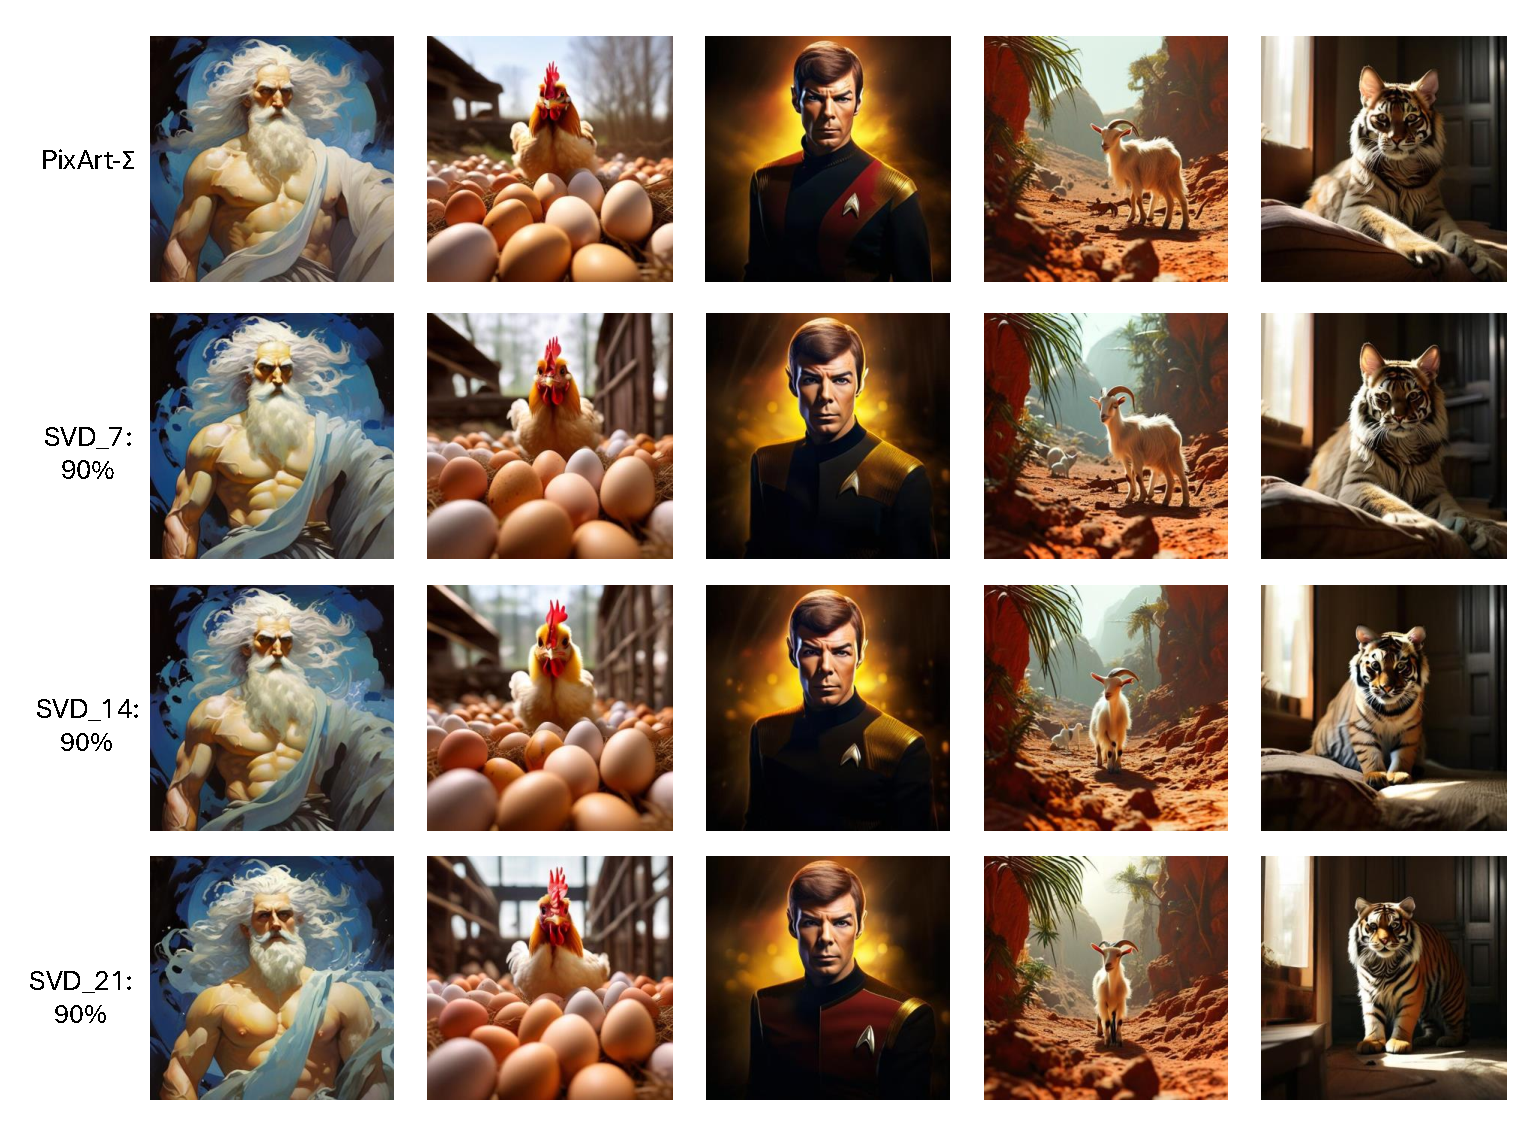
\includegraphics[width=0.7\textwidth]{images/Experimente/Compression_Schedul/ParameterDistribution_Appendix_model90.pdf}
	\caption[Qualitative Examples: Importance-Aware Rank-Adaptive Progressive Compression (90\% Model)]{Qualitative comparison of example images generated by models reduced to 90\% using the importance-aware rank-adaptive progressive compression schedule versus the standard progressive schedule (last row). The rows illustrate experiments utilizing a varying number of blocks targeted per iteration.}
	\label{fig:AppxCompressionSchedules90}
\end{figure}

\begin{figure}[H]
	\centering
	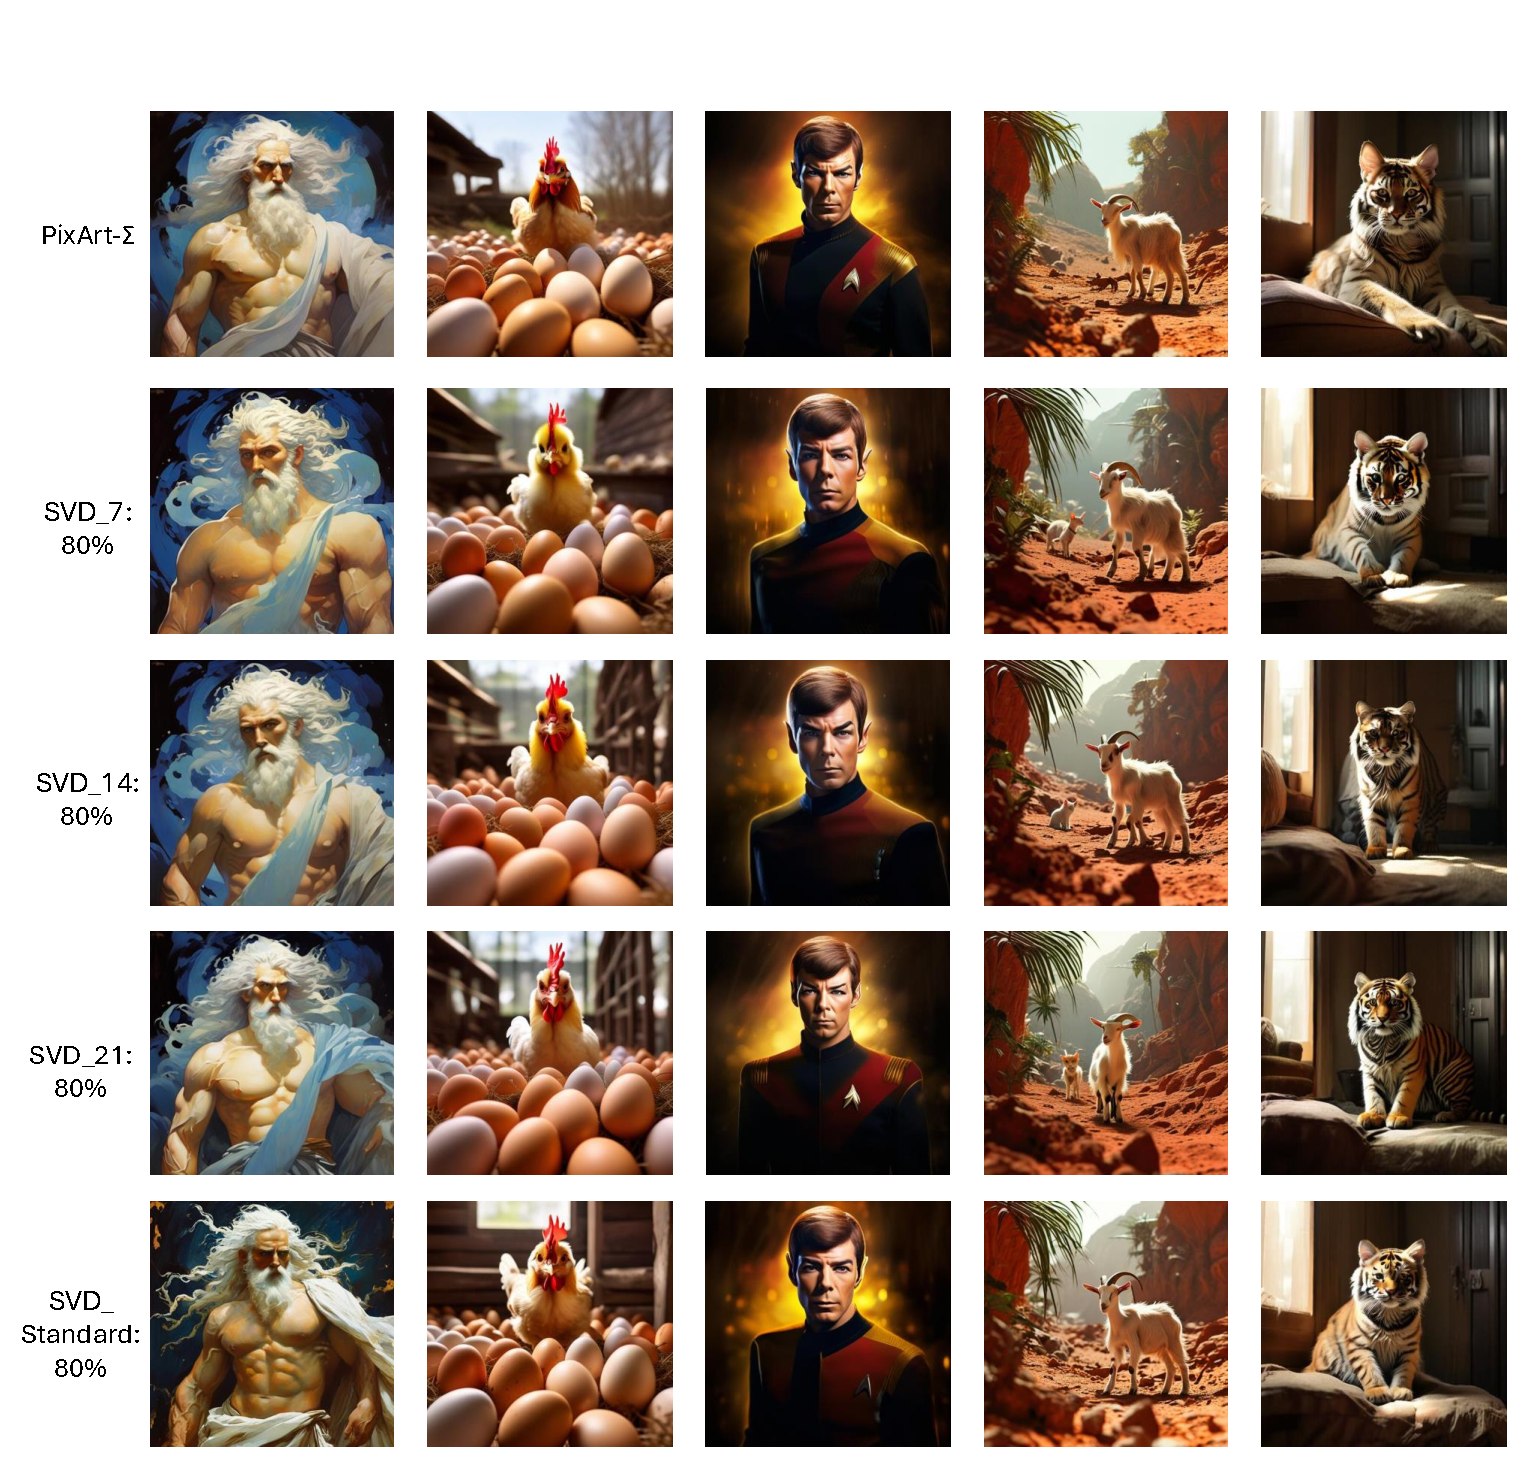
\includegraphics[width=0.7\textwidth]{images/Experimente/Compression_Schedul/ParameterDistribution_Appendix_model80.pdf}
	\caption[Qualitative Examples: Importance-Aware Rank-Adaptive Progressive Compression (80\% Model)]{Qualitative comparison of example images generated by models reduced to 80\% using the importance-aware rank-adaptive progressive compression schedule versus the standard progressive schedule (last row). The rows illustrate experiments utilizing a varying number of blocks targeted per iteration.}
	\label{fig:AppxCompressionSchedules80}
\end{figure}


\begin{figure}[H]
	\centering
	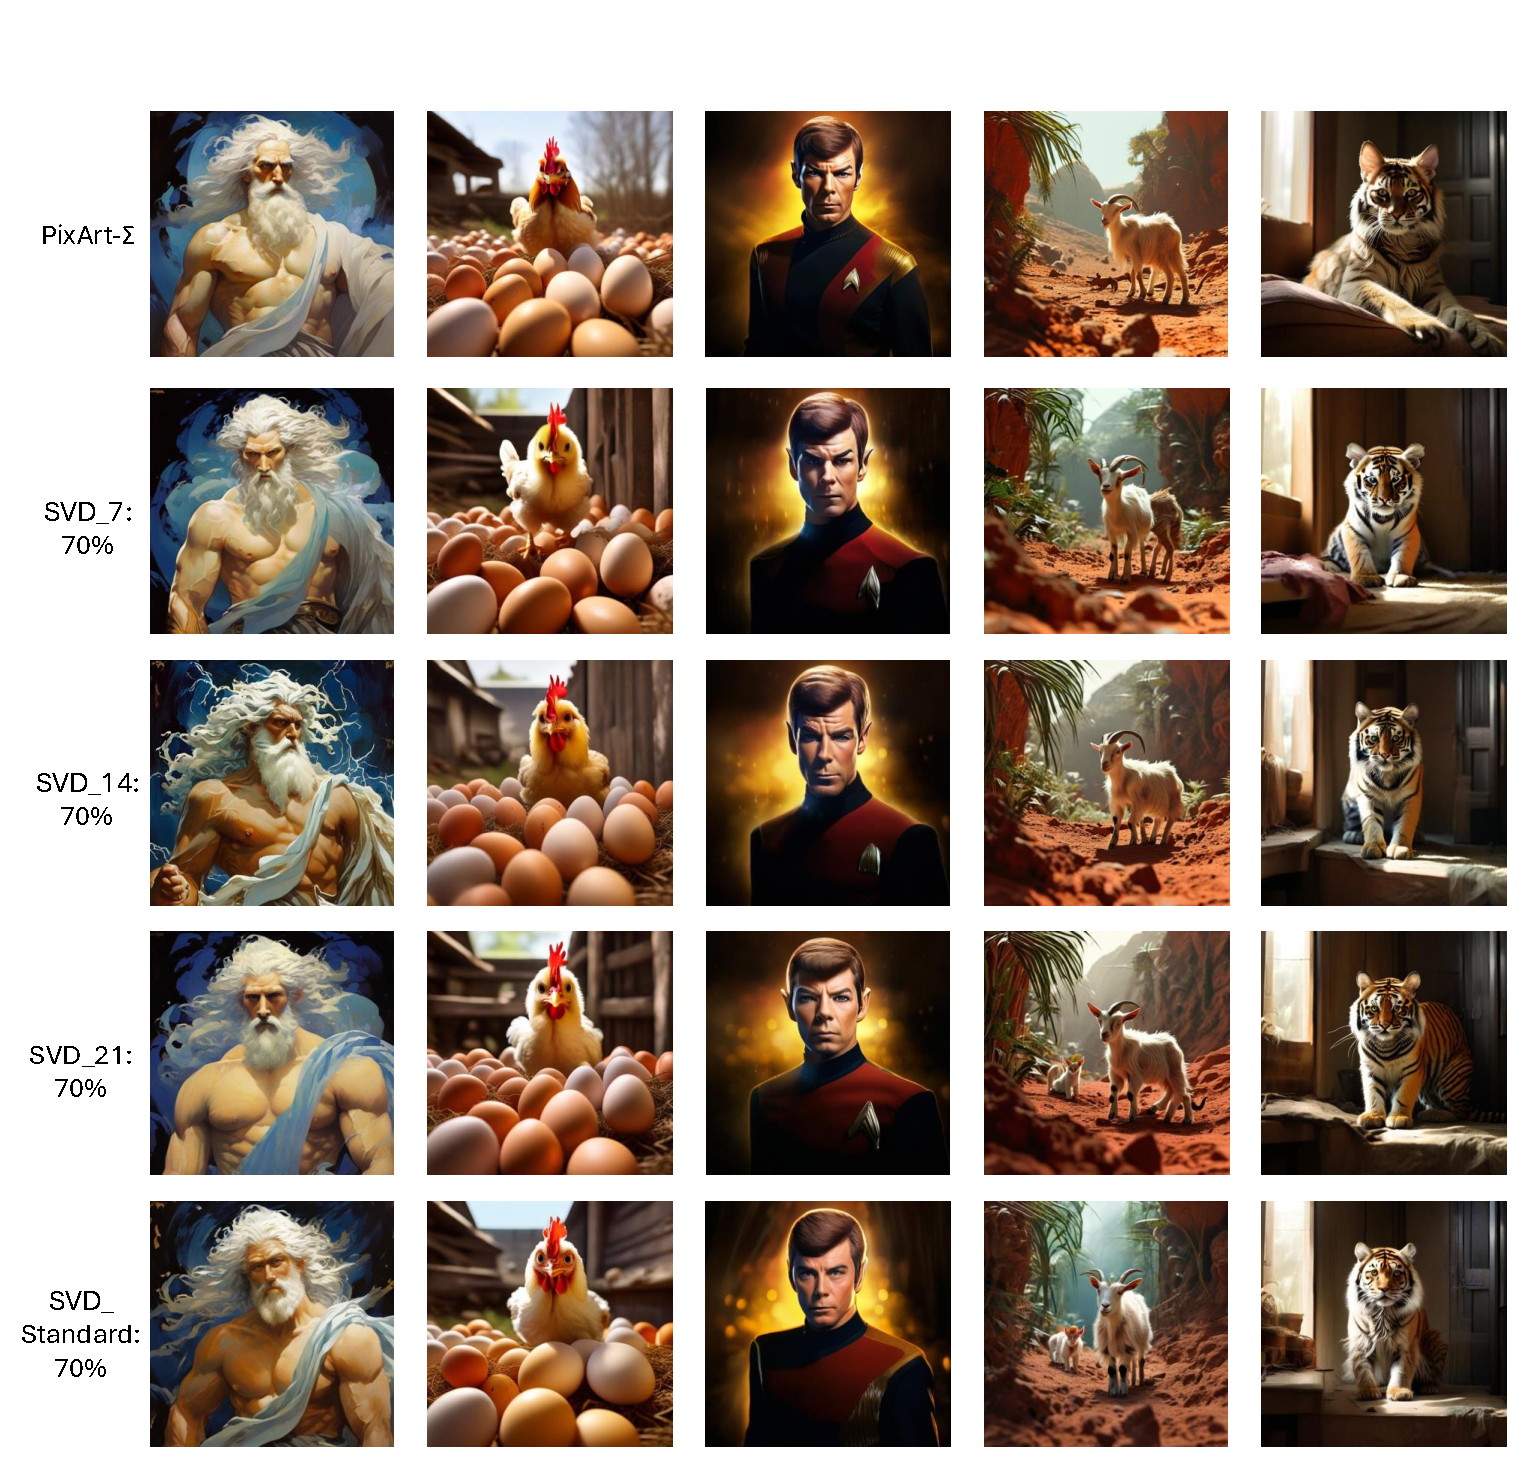
\includegraphics[width=0.7\textwidth]{images/Experimente/Compression_Schedul/ParameterDistribution_Appendix_model70.pdf}
	\caption[Qualitative Examples: Importance-Aware Rank-Adaptive Progressive Compression (70\% Model)]{Qualitative comparison of example images generated by models reduced to 70\% using the importance-aware rank-adaptive progressive compression schedule versus the standard progressive schedule (last row). The rows illustrate experiments utilizing a varying number of blocks targeted per iteration.}
	\label{fig:AppxCompressionSchedules70}
\end{figure}


\begin{figure}[H]
	\centering
	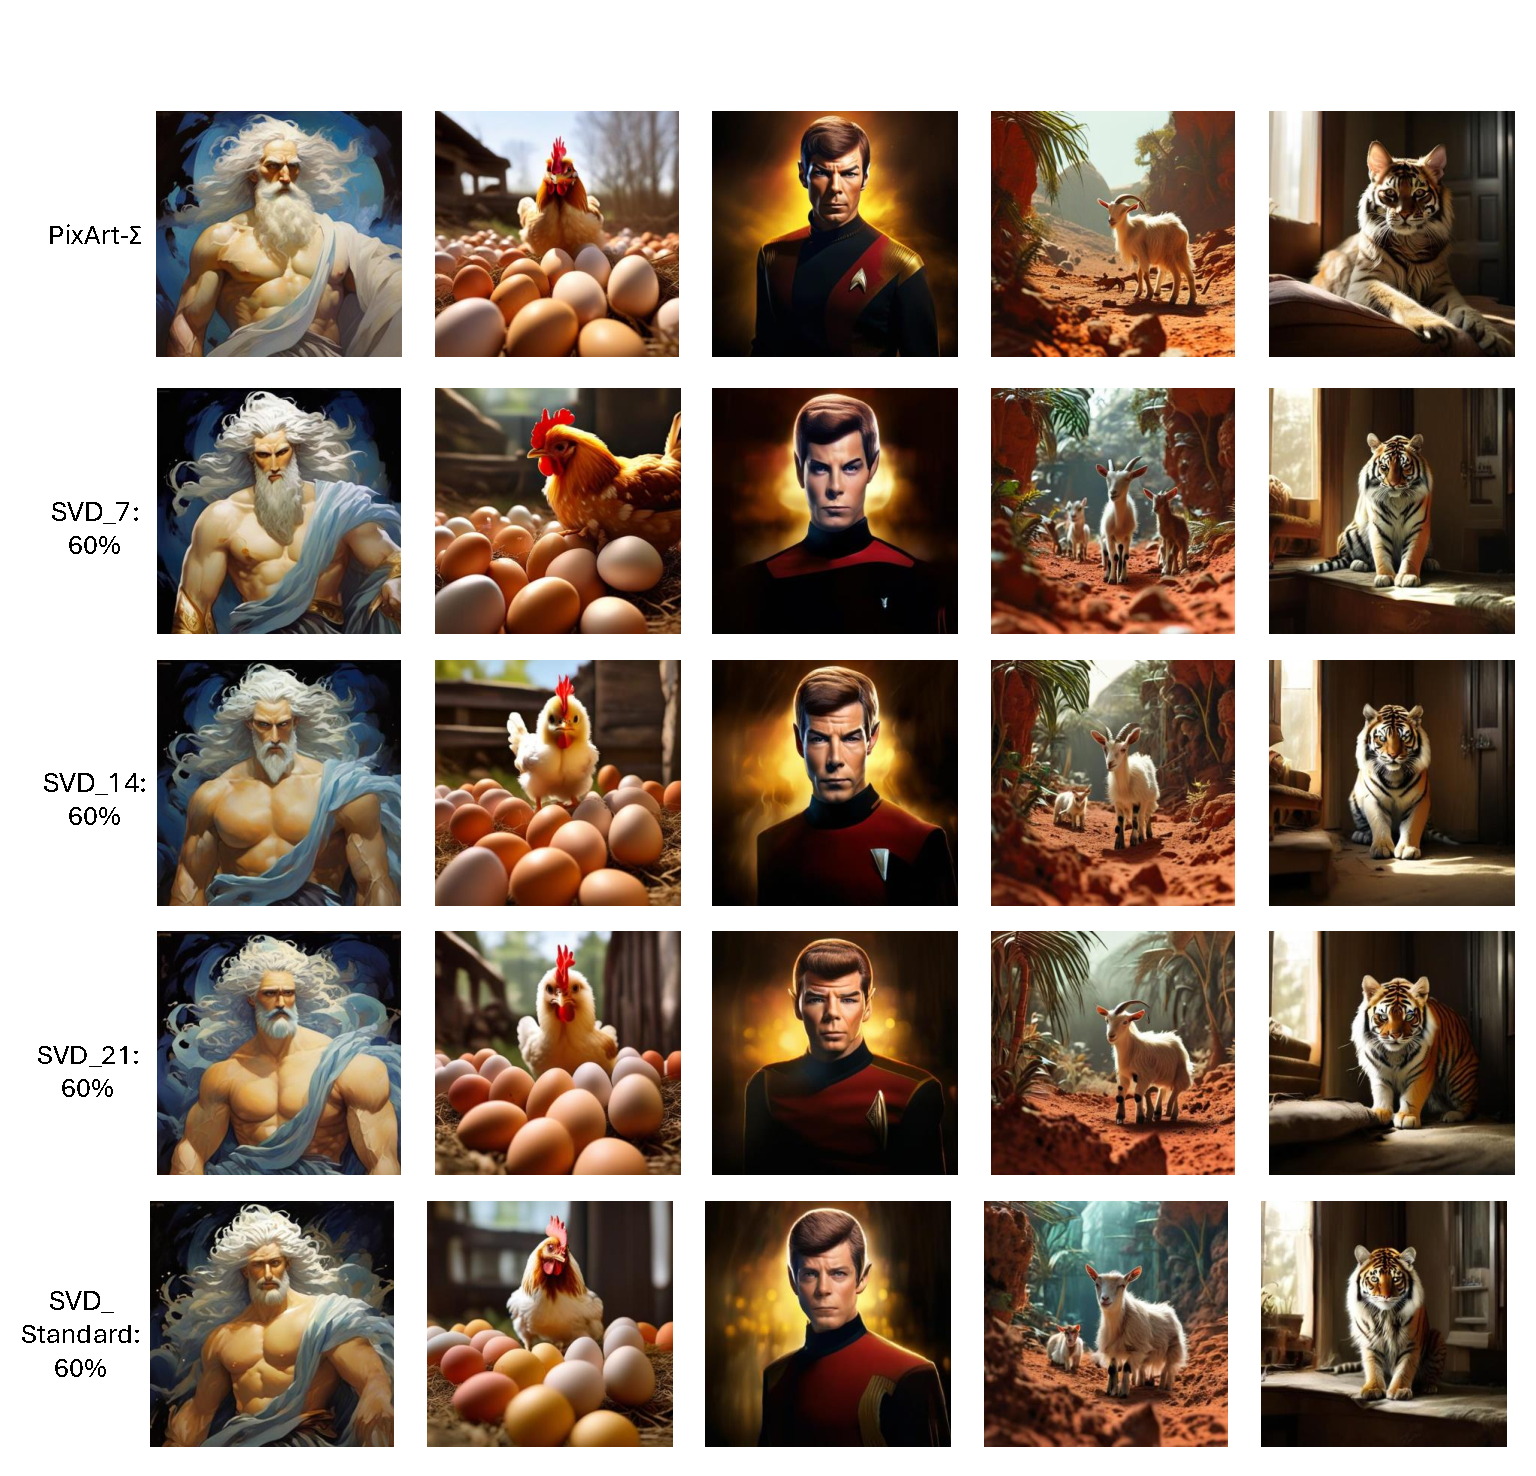
\includegraphics[width=0.7\textwidth]{images/Experimente/Compression_Schedul/ParameterDistribution_Appendix_model60.pdf}
	\caption[Qualitative Examples: Importance-Aware Rank-Adaptive Progressive Compression (60\% Model)]{Qualitative comparison of example images generated by models reduced to 60\% using the importance-aware rank-adaptive progressive compression schedule versus the standard progressive schedule (last row). The rows illustrate experiments utilizing a varying number of blocks targeted per iteration.}
	\label{fig:AppxCompressionSchedules60}
\end{figure}
